\chapter{Spread of the Neolithic through Central and Northern Europe} %13500
\label{ch:summedprob} 
Following on from Hambledon, this study takes a continental scale of analysis, taking as its source a data set of radiocarbon dates spread across Northern and Central Europe. The EUROEVOL data set \citep{Manning:2016fk} includes a variety of different types of data, for this study, only the radiocarbon section of the data set is considered. The difference in scale between this study and the last will enable a comparison of the problems and approaches of dealing with spatio-temporal data at opposite ends of the spectrum of scale. It is this comparison of spatio-temporal approaches and benefits of combined study across multiple scales that will enable this thesis to draw conclusions about archaeological analysis more generally. This study will enhance the broad problem space that is the spread of the Neolithic at the continental level, the interpretations at this level are generalising and reductionist, but that is no reason that they cannot be improved with the application of combined spatio-temporal analysis.

\section{Background}
The EUROEVOL data set \citep{Manning:2016fk} (or a similar precursor dataset) has featured in a variety of studies, such as \citet{gkiasta2003neolithic} and \citet{Russell:2004fk}. They used the data set to assess the method(s) by which farming spread across Europe, and from where. The conclusions from these studies have demonstrated a major axis regression, with an origin around Jericho about 10,000 years ago (calibrated) \citep{gkiasta2003neolithic}. These studies use methods such as isochron maps, taking a value (often the oldest) as a single value for each site in the database to show spread, and regression techniques to identify potential sources and rate of spread. In particular \citet{gkiasta2003neolithic} examined the relative importance of demic expansion, demic diffusion, and of trait adoption-diffusion as the mechanisms of spread by analysis of the pattern and rate of spread of farming. Such analysis focuses on the spatial component, taking a single uncalibrated year for each data point.

The data set has also been used in several studies to attempt to determine population levels, using variations on the summed probability distribution approach, examples include \citet{Shennan:2013fk}, \citet{TIMPSON2014549} and \citet{doi:10.1177/0959683614540952}. Such studies emphasise the temporal over the spatial components of the data, which reduces the richness of the data set. Here we shall first examine such approaches, assess their validity with respect to the available data, and examine the nature of the data set. Finally, the value of combined spatio-temporal methods at the continental scale will be demonstrated using a relatively simplistic model of the data.

\section{Summed Probability Distributions}
There has been considerable debate \citep{McLaughlin2016,steele_gkiasta_shennan_2004,Crombe:2004fk,SUROVELL20071868,SUROVELL20091715,BALLENGER20111314,Williams2012578,CONTRERAS2014591,Torfing2015193,Timpson2015199,Torfing2015203} and much use \citep{Shennan2013,Downey30082016,10.1371/journal.pone.0105730,PEROS2010656,HINZ20123331,WOODBRIDGE2014216,TIMPSON2014549,doi:10.1177/0959683614540952} over many years of the approach of summed probability distributions (SPD). The criticisms are either based around the underling theory of the approach, and what it is actually representing, such as \cite{McLaughlin2016,Torfing2015193,CONTRERAS2014591} among others; or on particular statistical issues, for example in the statistical modelling of taphonomic loss over time, e.g. \cite{SUROVELL20091715,steele_gkiasta_shennan_2004,BROWN2015133}. The proponents point to the statistical rigour and validation involved, and comparison to other data sets, such as pollen records, e.g. \cite{WOODBRIDGE2014216}. They are also keen to point out that as a proxy the results only show relative (not absolute) fluctuations, that large datasets are required to reduce the error margins, and that the time frames must be suitably large to remove fluctuations introduced by the C14 calibration curve \citep{Timpson2015199,TIMPSON2014549}.

\subsection{The Methodology}
The approach was pioneered by \citet{10.2307/281060} who defined the underlying theory, that ``the number of dates is related to the magnitude of occupation'' \citep[55]{10.2307/281060} by which he means that larger populations create more material, so more will survive in the record, leading to more samples being dated, therefore a sum of radiocarbon dates will result in greater values for times when the population is larger. This is underpinned by three clear assumptions \citep[56]{10.2307/281060}:
\begin{enumerate}
\item A large population deposits more material (specifically more carbon datable material)
\item The surviving material is proportional to the original
\item Carbon dates are representative of the preserved material 
\end{enumerate}
Rick states that as biases interfere with these assumptions, the method can only produce relative measures of occupation, otherwise it would be capable of producing absolute measures. Rick simply sums the number of dates falling within specific intervals \citep[61]{10.2307/281060}.

The approach taken by modern studies is methodologically much more sophisticated, an example with a good description of the method is \citet{TIMPSON2014549}. For full details see Appendix one of that publication, \citep[555]{TIMPSON2014549} some notable additions to the method include the binning of dates, and averaging of dates in each bin, so effectively each site-phase (or bin) only contributes a single date to the final sum. The summed probability distribution is then computed over the site-phase averages, and then transformed so the resultant values all sum to one - i.e. transformed into a probability. Another significant addition is the generation of a simulated data set, to go alongside the real one. A C14 data set is simulated, using an exponential model (the null model) to guide the random sampling, the number of dates generated is the same as the number of bins, a summed probability distribution is then calculated for the simulated data.  A further addition is de-trending of the SPD, using a method called the `local Z-transform' \citep[556]{TIMPSON2014549} applied to remove short term wiggles introduced by the calibration curve, and also the long term exponential trend of the null model. Finally a global p-value is used to assess the significance of the model, with deviation from the null model signifying a deviation from anticipated population levels.

The method is credited with being able to identify population boom and bust patterns around the start of the Neolithic, for example in England and Wales (without Wessex) ``a boom following the arrival of farming at c.6000 BP followed by a crash down to a level little more than half the preceding peak. The population remains at this relatively low level for nearly 800 years'' \citep[554]{TIMPSON2014549}. Here the results are interpreted by visual examination of the curve on the graph, although statistical tests are used to identify the areas deviating from a null model. The interpretation of such values directly as ``population'' is explicit, although the technique is not able to provide population figures. Similar results have also been observed by \citet{Shennan:2013fk} and \citet{Stevens:2012fk}. \citet{CREMA20171} provides the only extension to the technique into the spatial dimension, considering how deviations from the null model are distributed spatially.

\subsection{The Criticisms}
The method has not been without its criticisms, these can be roughly split into two groups, those that focus on methodological issues and those that are more concerned with theoretical concerns. Researchers have attempted to correct for methodological issues with more statistical techniques, but theoretical problems are more fundamental.

\subsubsection{Methodological Issues}
Methodologically there have been a few key areas which have seen significant work to alter the original process. These focus on the affects of the calibration curve, such as \citet{BROWN2015133}, the taphonomic loss of sites over time studied by\citet{SUROVELL20071868,SUROVELL20091715} and sample size, \citet{Williams2012578}.

\paragraph{The Calibration Curve}
The calibration curve exerts a strong influence over the output summed probability distribution, with the peaks and troughs either concentrating samples in certain date ranges, or spreading them out over others. This non-linear relationship is responsible for introducing artificial structures that are time-dependent into summed probability distributions \citep[141]{BROWN2015133}. \citet{BROWN2015133} advises against trying to investigate short-run demographic processes using such methods, due to the difficulty in distinguishing between demographic structures and non-demographic ones with small samples and the absence of clear recommendations over necessary sample sizes \citep[142]{BROWN2015133}. The effects of the calibration curve have been observed in studies such as \citet[137]{McLaughlin2016}. To counteract these artificial structures several authors recommend that results are presented with a moving average trend line \citep[584]{Williams2012578} which \citet[143]{BROWN2015133} have recognised as a form of kernel density estimate. The outcome of applying this correction is that artefacts in the resultant SPD, which might come from the calibration curve are averaged out, this technique does not discriminate by the source of the artefact, so will smooth the result regardless, potentially smoothing out features from the original distribution.

\paragraph{Taphonomic Loss}
The issue of taphonomic loss has received considerable attention, \citet{SUROVELL20071868} examined the issue of site loss over time, demonstrating that older sites were less likely to survive, leading to fewer being dated. They demonstrated through simulated data sets that an exponential SPD would be generated, simply due to the taphonomic loss of sites. They concluded ``it is unlikely that a true demographic signal can be easily extracted using frequencies of dates or sites alone''  \citep[1874]{SUROVELL20071868}. As with calibration effects, statistical methods have been proposed to remove such taphonomic effects: \citet{SUROVELL20091715} use the volcanic record to develop a global model of taphonomic loss. However such a correction has its limitations, temporally it is limited to the age of the deposits used for constructing the model. \citet[584]{Williams2012578} state that such corrections don't work for dates over 15,000 years ago, and that ``an assumption of exponential time-dependent taphonomic loss may not be strictly valid'' \citep[586]{Williams2012578} this last point leads to their concern that such corrections may obscure real trends in the data. There have also been concerns over the validity of such a global correction, \citet[1321]{BALLENGER20111314} note that such a method does not account for large-scale changes in deposition and erosion through time. They create an alternative model from alluvial deposits, stating  ``our model is fundamentally different from the volcanic-based model because we assume that radiocarbon frequency distributions are based on what researchers sample, not what exists, and the nature of the stratigraphic record'' \citep[1322]{BALLENGER20111314}. Crucially \citet[1322]{BALLENGER20111314} note that there is a sparsity in the dataset at the end of the series, they draw attention to the fact that there is only one 40,000 year old radiocarbon date, and that while this might be expected given the model of taphonomic loss, the sample size of one is not  sufficient for model construction. In addition, \citet[593]{CONTRERAS2014591} note ``it is assumed, unrealistically in our view, that in large data sets, taphonomic filters will not discriminate between regions and site types'' this is a central tenet of using a global model on a dataset spanning a large geographical area, and is also a point raised by \citet{BALLENGER20111314} when they compare records between different areas. This touches upon a key issue in the SPD discussion, does the size of the dataset mean that a broad, global model is applicable? These studies argue to the contrary, and that local, more nuanced model should be used instead. However across a very large geographic area, it might not be possible to construct such local models for the whole study area.

\paragraph{Sample Size}
As \citet[142]{BROWN2015133} notes there is little in the way of reliable recommendation for adequate sample sizes. However \citet{Williams2012578} have performed an analysis of samples for SPD, recommending a minimum sample size in the region of 200-500 samples \citep[580]{Williams2012578}. They also note that there are assumptions made of the sampling strategy that are often not met \citep[593]{Williams2012578}. They assert  ``multiple small nonsystematic samples from a large assemblage of sites constitute a quasi-random sample of regional trends in occupation'' \citep[580]{Williams2012578} this also relates to the the key issue touched upon above, that of scale, is it valid to accept the assumption, that lots of small non-systematic samples when combined can be treated for statistical purposes as though they are, in the words of \citep{Williams2012578} ``quasi-random''? Another important factor of sample size, often not touched upon is that modern methods usually equalise sites (e.g. \citealp{TIMPSON2014549}) in this case, is it the number of samples, or the number of sites which is key? \citet{Torfing2015193} notes this, and asserts that it is in fact the number of sites that is important \citep[197]{Torfing2015193}. This conclusion is consistent with studies that make use of simulated data sets, as they will only generate one per site. So the recommendation of 200-500 samples should actually be 200-500 sites.

This brief overview has examined the key methodological debates surrounding the technique, clearly these debates are still open, with potential solutions being proposed, and subject to debate and criticism in their own right, as is required to refine the technique. The underlying subtext of most of this debate is that there is a valid solution to such problems, it is simply a matter of finding and validating it.

\subsubsection{Theoretical Issues}
Such a view contrasts that of the more theoretical criticisms, which question the very validity of the method itself, for example \citet[1321]{BALLENGER20111314} leave nothing to the imagination with their statement: \begin{quote}``we are not convinced that archaeological radiocarbon dates are an accurate proxy for the abundance of people or that relative changes in human demographics can be extracted from radiocarbon frequency distributions''.\end{quote}

\paragraph{Research Bias}
\citet{BALLENGER20111314} are primarily concerned about the issue of scientific bias from research focus. In the particular study area of the American Southwest, there was considerable research focus on the Clovis, having a total of 118 samples, whereas dates from the Hohokam interval had only been recovered from two cultural resource management projects \citep[131]{BALLENGER20111314}. The authors of that paper are clear that such disparity is unlikely to be due to the original population sizes, and are the result of very specific research focus in the area. \citet{McLaughlin2016} consider such biases in the context of Neolithic Ireland, identifying important trends, such as excavated sites being mostly close to contemporary urban centres, or along major infrastructure routes; or the fact that certain types of sites, being made of stone are still visible in the landscape and have received much more research focus due to their visibility than other types of sites; or the bias of development led excavation to natural route-way locations \citep[139]{McLaughlin2016}. \citet{Torfing2015193} also investigates this bias, he examines the influence a single researcher can have on the SPD, in this case S. H. Anderson \citep[196]{Torfing2015193}, and while this influence is not quantified, \citep[200]{Timpson2015199} it does demonstrate that an individuals research agenda can have a clear impact on SPDs. 

Another example of this is from the study by \citet{PALMISANO201759}. There is clear recognition that for certain periods the SPD approach can be affected by how archaeologists conduct their research, in this case during the Roman period the reliance by archaeologists on typo-chronological schemes creates a massive underestimate of the population \citep[66]{PALMISANO201759}. This is the first time that at least one of these authors have recognised a specific point in time and space where the SPD approach is demonstrably invalid. It is of crucial importance, as this is the crux of the argument in \citet{Torfing2015193}. It calls into question the validity of applying such models over large areas of space and time, without conducting a rigorous examination of the source dataset and the biases which may be present therein. It also provides a good case study of the kinds of effects the techniques chosen by archaeologists can have on the underlying data set. This is unlikely to be an isolated situation, for example radiocarbon dates of the British Iron Age are affected by the Hallstatt plateau, so less material is submitted for dating for this period than for other periods.

\paragraph{Variability among site types}
\citet{Torfing2015193} also examined the effect different monument classes can have on the SPD, first calculateing SPDs of all sites from a dataset, then an SPD from only settlements and middens, and finally an SPD from dates only from settlement sites \citep[194]{Torfing2015193}. These latter two excluding the very visible (and therefore investigated) Neolithic monuments, the results of which demonstrated that the types of sites included in a dataset have an impact on the resultant SPD. This is an important consideration for studies of the Mesolithic-Neolithic transition in Northern Europe, as monuments make up such a large part of the Neolithic record than the Mesolithic. \citet{McLaughlin2016} demonstrated a similar point by focusing exclusively on pit-and-spread sites, on the basis that these are present for many periods, and are the result of settlement activity \citep[141]{McLaughlin2016}. These results were compared with SPDs of all sites, and used to control for the high visibility of some site types. The authors were cautious about inferring demographic events as the causes of fluctuations in the SPD, and also looked at (somewhat limited) genetic evidence \citep[142]{McLaughlin2016} that would seem to imply that demographic changes were not responsible for changes in the pit-and-spread SPD. They conclude that such an approach can ``illustrate the problems of taking the archaeological record too literally in terms of demographic modelling'' \citep[143]{McLaughlin2016} and ``far from seeing a boom and bust of prehistoric populations at this time, we see ... a record of cultural change'' \citep[144]{McLaughlin2016}.

\paragraph{Cultural Change}
A third potential source of problems for SPDs might broadly be termed changes in culture. Torfing analyses this in terms of subsistence strategy on the basis that shell middens are indicative of a certain subsistence strategy, but that they also offer a much greater possibility of extracting radiocarbon dates, due to better preservation \citep[196]{Torfing2015193}. Effectively what he is arguing is that specific patterns of subsistence leave greater traces in the archaeological record. This is very similar to \citet{CROMBE2014558} who instead focus on patterns of mobility, they have shown how reduced mobility at the end of the Mesolithic, due to increased dependence on aquatic resources, leads to fewer sites, crucially without significant demographic changes, resulting in fewer samples being dated by archaeologists today \citep[560]{CROMBE2014558}. This issue is summed up by Torfing: ``while it is true that the 14C-dates from archaeological sites originate from past human activity in one form or another, it is noway clear that all past human activity will leave a comparable amount of datable material''  \citep[193]{Torfing2015193}.

This is just a coherent sample of the criticisms, other authors have taken a variety of novel approaches, such as \citet{CONTRERAS2014591} who constructed simulated datasets from known, historical population fluctuations. Effectively they have modelled the scenario backwards, producing datasets to match known population fluctuations, and then attempted to see if these changes were visible in the radiocarbon record. In this case it was not successful, with the authors concluding: \begin{quote}``both advocates and critics of a `Sum' approach might hope that simulation studies would produce baseline criteria ... Unfortunately, the abundance of variables ... and the irregular population distributions that we are trying to reconstruct ... mean that any such rule of thumb is likely to represent wishful thinking rather than rigorous evaluation'' \citep[605]{CONTRERAS2014591}.\end{quote}

These criticisms make two broad points, firstly that past human activities do not generate comparable amounts of radiocarbon datable material, different subsistence patterns, mobility patterns, and changes in material cultural will impact the quantity of material deposited. A key demonstration of this is pottery, while not radiocarbon datable itself, burnt food residues, when found, can and are radiocarbon dated. Societies which do not have pottery, therefore will produce no such datable residues, not because they did not eat, or because there were necessarily fewer people, but because food containers were likely made of organic materials, which have not survived. This is a key assumption omitted by Rick, that to compare societies across space and time, they must produce similar quantities of datable material per head of person. This also includes that societies will expend time and energy in different ways, so building (highly visible monuments) will result in the creation of concentrated datable material, where as moving around a landscape will result in a different quantity, over a more dispersed area. This brings us to the second class of criticism, differential investigation by modern researchers. Highly visible monuments are much more likely to be investigated than invisible ones, archaeologists tend to focus on certain sites, and geographic areas, they also choose to have certain samples data, in particular to answer research questions on boundaries between distinct phases. Such factors compound one another across the dataset, and may occur very broadly, for example archaeologists dating strategies will likely exert an influence over a country wide radiocarbon dataset, and potentially further afield. If such effects are not explicitly accounted for the resultant SPD will be skewed. In a guarded critique \citet{whittle2018times} splits the problems with the technique into three categories: uncleaned databases, the summing of probability distributions, and the assumptions behind the link between radiocarbon dates and population levels.
 
\subsection{Validating the Method}
\citet{Timpson2015199} provides such a reply to the criticisms described above, specifically of Torfings criticisms, but also more generally. 

\citet{Timpson2015199} are critical of approaches that reduce the sample size as this can increase the sampling error, instead they recommend that it is better to include data with known biases, to create a larger data set on the basis that ``the combination of many different biases will approach a random error'' \citep[201]{Timpson2015199}. However this claim is only backed up by a vague reference to the ``Law of Large Numbers'' and as Torfing notes, any biases that are systematic are likely to affect the resultant SPD as they will not be masked by other, more random errors. This returns us to a fundamental question, already encountered, can large archaeological data sets of non-systematic samples be treated, for statistical purposes, as random, due to their size? This criticism of sample reduction is also contra \citet{TIMPSON2014549} who claim that ``the statistical power to detect significance with sample sizes as small as 12 dates across 4000 years'' \citep[552]{TIMPSON2014549}. Clearly it cannot be the case that both these points are valid, either it has the ``statistical power'' or it requires large quantities of data.

They also reject entirely the criticism of activities producing incomparable quantities of datable material, by providing the rather contrived example of record players, replaced by cassettes, then CDs and finally iPods \citep[201]{Timpson2015199}. The key problem with this is that while each of these replaces its predecessor, so in principle it could be a proxy for demography, in reality we would see increases at each step (until the arrival of iPods - which have no removable media), this is in fact due to increasing affluence, a variable unrelated to population size. As Neolithic monumentality does not have a predecessor in the same way, this argument does not support the applicability of SPDs to the Mesolithic - Neolithic transition. In support of their position, \citet{Timpson2015199} cite Ricks assumption that  the amount of human activity is a proxy for population and concludes by recommending that all data be included as this increases the sample size.

There are two key methods that are often used to provide a validation of SPD results, the first is comparison to null hypothesis, introduced above, and the second is comparison to other proxies of population.

\subsubsection{Null Model Hypothesis Testing}
Of crucial importance, according to \citet{Timpson2015199} is the inclusion of a null hypothesis test \citep[200]{Timpson2015199}, a model of what we might expect past population to look like. Statistical tests are used to measure how closely the calculated SPD matches the null model, providing a quantitive basis for acceptance or rejection of the null model. Such null models often include a correction for taphonomic loss, and an expected long term increase in population, however as we have seen above there are concerns about such taphonomic models. Regardless of the particular null model chosen, this form of test provides a more rigorous examination of the SPD than a mere visual inspection, and a numerical basis for comparison across SPD studies. Unfortunately, while \citet{Timpson2015199} are valid in their criticism of Torfing, they merely draw attention to this, rather than attempting to advance the field by calculating such metrics of Torfings studies, which ironically is similar to another of their criticisms of Torfing, that he is only finding flaws, and not providing solutions.

While very few would argue for a visual inspection as a favourable method of examining statistical results to a quantifiable approach, there are several elements of the null hypothesis, or model to consider. Firstly how it is generated, and then how it is used to validate the SPD results. Null models are generally generated to account for both taphonomic loss and for a general long term exponential population growth, for example in \citet{TIMPSON2014549} where an exponential model is chosen. Having examined above some criticisms of such a global model of taphonomic loss, it is clearly any null model generated in such a way may not be applicable across a study area and time period. Secondly, what does comparing the SPD to such a generated model actually tell us? It is clearly assuming that a doubling of population should result in a doubling of radiocarbon datable material being deposited and that the proportion recovered and dated would therefore also double. Perhaps unsurprisingly the null model tests used in SPD studies encapsulate the fundamental (and controversial) assumptions of the SPD approach. There is a kind of circularity here, for the null model checks to validate the use of the SPD approach it is necessary that the basic assumptions outlined by Rick are valid. If we challenge the assumption that large populations generate more radiocarbon datable material, and instead postulate that the amount of radiocarbon datable material produced is a function of population size and cultural practices, such that changing cultural practices can result in large populations producing less than smaller ones. Then the null hypothesis tests, using an exponential model, no longer provide a valid metric for assessing whether an SPD deviates from what we might expect given a steadily growing population. Clearly there is scope here for much more nuanced null models, that could be used to compare a range of environmental and cultural factors affecting demographic changes over time.

\subsubsection{Comparison to other data sets}
SPDs have been compared to a variety of other data sets: \citet{WOODBRIDGE2014216} compare an SPD to an off-site pollen record for Britain. The conclusions of this approach show that during times of (expected) increased population change there are also corresponding changes to the pollen record. Specifically at the start of the Neolithic \citet{WOODBRIDGE2014216} note a significant population growth occurring alongside a change from deciduous woodland to semi-open arboreal land-cover \citep[219]{WOODBRIDGE2014216}. While this comparison might show correlations between the two metrics, it does not show any causation, in fact if we assume (for the sake of argument) that the SPD is merely showing an increase in archaeological dating at the start of the Neolithic period, the correlation is still interesting and expected, due to the arrival of farming. Crucially the comparison of the two in no way supports the validity of the SPD approach.

\citet{PALMISANO201759} performed a direct comparison of SPD to settlement counts, claiming ``broad agreement in the demographic trends produced by the SPD of radiocarbon dates and the other five related settlement indices'' \citep[68]{PALMISANO201759}. This would appear to involve some artistic license. In particular, the authors note ``here is general agreement among all proxies in identifying an increase of population in the Early Neolithic, in the Eneolithic, in the Final Bronze Age/Iron Age and a last demographic boom during the Roman Period'' \citep[70]{PALMISANO201759} however the last in this list of claims seems spurious, as the authors clearly note that during the Roman period the SPD ``massively underestimates a widely-agreed and widely-evidenced boom in population'' \citep[66]{PALMISANO201759}. This would mean that across an 8000 year time period there is agreement for three periods, lasting very roughly for a few hundred years each - not quite the broad agreement claimed, and certainly calling into question the assertion that the SPD ``can be regarded as a robust proxy for modelling population fluctuations through time'' \citep[68]{PALMISANO201759}. The only measure of equivalence between the proxies is a global Pearson's correlation and while it may show a general agreement, hides the significant fluctuations between the different approaches. 

The reasons for such agreements should be quite clear, what the SPD approach measures is not population, but activity, as a proxy. This activity is based on dates from those sites excavated, so it is unsurprising that it would correlate with a simple count of sites, this is also the same source for the aoristic and random approaches, and crucially the random SPD approach, which has the greatest correlation, however that is because the SPD data is used to seed the aoristic randomised start dates, creating a circularity within this technique \citep[63]{PALMISANO201759}. The technique whose data is most removed from the data used in the SPD, and would therefore have the least bias, is the summed settlement area, as this didn't just use excavated sites. It is also the proxy with the smallest correlation across the whole date range. This is not to say that it is a good proxy in and of itself, there are many variables that could affect it, but as all the other techniques are connected in at least one, and potential several ways, it is not surprising they show a correlation. It is telling that the most impartial of all tested methods shows the least correlation. What the authors have not done is attempt to quantify how much we might expect a correlation given the same source data and compare this to the actual correlation.  

\subsection{Further concerns with the method}
Following the review of criticisms and validations of the method several key issues appear that deserve further examination.

Ricks first assumption, that ``a larger population deposits more material'' \citep[56]{10.2307/281060} is analysed by \citet{Torfing2015193,CROMBE2014558}, both clearly demonstrating the effect on the SDP of different types of culture, where some are more archaeologically visible and so make up a greater part of the available record. Here Rick is stating that the quantity of material is directly related to the population size, stated algebraically this could be written as $\sum m \propto p$ where m is material deposited and p is population size. This requires the material deposited per person, on average, to be roughy equal, across time and over space, implying a consistent uniformity or rationality as the basis for the behaviour of individuals, the \textit{Homo oeconomicus} of \citet[197]{Shennan:1991uq}. The questions is whether that is an acceptable assumption. For a large scale model it may be appropriate to accept such assumptions, even though we do not believe that they hold at an individual level, as \citet{Shennan:1991uq} points out economists and ecologists routinely make such assumptions. What \citet{Torfing2015193} and \citet{CROMBE2014558} show is that changes in cultural practice lead to differential quantities of material being produced, specifically material that is radiocarbon datable, this could be written as $\sum m \propto c(p)$ i.e. cultural process can be seen as a transformation of the material produced at the population level. Specifically the Neolithic introduced new material that can be carbon dated, such as cereals, domesticated animals, residues on pottery it also introduced changes to lifestyle such as the building of monuments and increasing sedentism, which result in a greater potential of material being recovered. 

The final assumption of \cite{10.2307/281060}, that radiocarbon dates are representative of the material created by a population. This assertion does not appear to have been tested or proven at all, despite it's importance. It also places radiocarbon datable material in a privileged position, without any evidence or explanation. Rick's other two assumptions could be taken as a basis for using sherd counts (or weights) or flint counts, or counts of any other form of material culture as a basis for inferring past populations. Of course to asses the spread of the Neolithic these may be problematic, as there is a clear change in culture, especially in Britain, where the introduction of pottery is tied with the start of the Neolithic. This change in past material practice would clearly bias the results of a method using ceramics as a population proxy. Is radiocarbon datable material exempt from changes in past cultural change? This seems unlikely, but without a reason or evidence for the use of radiocarbon datable material over other forms, there is a question mark over its pre-eminence.

The other issues relate to the analysis of the EUROEVOL data set in particular but would apply to other analytical approaches as well. The use of the SPD method simply provides a convenient example to use to analyse these issues. They are concerns that are fundamental to the analysis of such data sets. Before undertaking any further analysis using this dataset it is important that these issues are explored and understood.

\subsubsection{Big Data}
The EUROEVOL data set is large, has been subject to various biases, is not a random sample and its underlying true distribution is unknown. It is exactly as \citet{doi:10.1177/0162243916671200} describes archaeological data: fragmentary and incomplete, punctuated by gaps and absences. \citet{Timpson2015199} argue that they can get around these issues with a large enough data set, that it will approach a random sample. The statistical rule they invoke for this magic is the ``law of large numbers''.

There are in fact several such laws, defined with mathematical specificity. The vague notion employed here would appear to be using a heuristic along the lines of: as the number of samples increases the average of the observations approaches the expected value. Firstly, such a rule would clearly depend on each sample being unbiased, for example if we attempted to employ the above law with regard to dice rolls, if our dice is weighted, no matter how many rolls we make the average of the observations will be skewed. Another requirement is clearly that each repeated observation takes place under identical conditions. Otherwise there is a clear potential for bias to be included at this stage, which would cause the observed average to deviate from the expected. Effectively this would mean the only variable in the process should be the observed value. Such a rule is clearly very valuable under these conditions, however these conditions make such a law more suitable to the kind of data gathered when conducting controlled laboratory experiments. 

Moving on from the premises, let us consider the subject of this law, the samples or observations. With the values of dice, an observation is straight forward, it is a single roll. In the case of the summed probability distribution studies examined above, the EUROEVOL data set is a (partial) record of the prehistoric population (according to the SPD methods proponents). Each record in the data set is therefore an observation on the original distribution, the roll of a dice. Population fluctuates across space and time, under this method each observation contributes to the population record across its probability distribution, potentially a large span of time. Each observation therefore being a specific dated event, not an independent observation on the same original distribution, but a biased observation on a different (albeit related) distribution. Under the law of large numbers as we make more and more rolls of the dice, the result will trend to the average value. In the SPD we are (indirectly) summing the number of events, the number of observations and not calculating their average. This is very different to what the law of large numbers describes. 

One of the final elements of the method is to normalise the values, so that they sum to one. This is being performed on the sum across the average values for all of the bins of dates. This would be the same as normalising each bin average, and summing the resultant probability values, at which point each bin (or site-phase) contributes a total weight (across its distribution) of one due to the normalisation. If this value were to be attributed to a single year, that year would take the value of one. The method becomes effectively adding up the number of bins, to determine the population of a year. To continue this thought experiment, if each observation on the data returned a specific year, the method would then become add all the dates up on a per year basis, and get the average values for each year per bin. Divide this value by one, then sum the values across bins. Ultimately the method reduces to adding up the numbers of dates, the averaging and normalising reduce the disproportionate effect of well dated site phases. Of course, in this case each date is clearly not a sample of the underlying population distribution, it is simply a single date, which has the arbitrary population value of one. The final population is based on a sum of these values, a sum of the observations. The law of large numbers is based on the average of values of observations, the SPD has been shown above to reduce to the number of dates. If the underlying distribution is biased, for example by a focus on certain periods, this could lead to more dates being available for certain time values, which would lead to the bias transferring through to the final value. Adding more dates does not dilute the bias, if the additional dates also include the same biases, it will only exacerbate the effect. Ultimately, adding more dates simply increases the sum, rather then refining the average.

At this point, proponents of summed probability distribution might suggest this line of argument is a straw man, pointing out the values are averaged per bin. Let us consider this, each calibrated radiocarbon date provides a probability distribution for the date of a particular event. As we have seen in the previous chapter, many events per phase is most useful when combined with a chronology. So what can the average of multiple dates provide? As each is for a potentially independent event and some may be residual or intrusive, the average simply provides us with a middle value from the partial, biased data set we have, weighted by those events which create more material that is datable, and are most interesting to archaeologists. If we were dealing with absolute dates, this might be useful if we did not know exactly when a short lived phase began and ended, as the average value would give us a likely locus for the phases use. However radiocarbon dates already include a measure of uncertainty, so averaging this is probably a less useful exercise than building a bayesian model to provide start and end boundaries for a phase. In terms of the law of large numbers there are two points to consider, firstly from the perspective of the values as dates, this is an average of multiple, different events (not multiple observations on the same event) so adding more dates to an average in this way will not trend to the true value of a site phase. Secondly from the perspective of summed probability distribution, the average is simply computed at this point to provide an average value for the date of the site phase. Due to the normalisation, the law of large numbers should really be invoked on the site phases (rather than radiocarbon distributions) as we have seen above, this reduced to counting numbers of phases. Fundamentally adding more dates does not make the date of each bin more accurate, and due to the normalisation does not increase the number of observations used to construct the final summed probability.

\subsubsection{Null hypothesis testing}
Despite this the proponents of the SPD method may point to the simulated data set, and null model test as proof of the validity of the method. That the SPD broadly follows exponential long term growth \citep{Shennan:2013fk} when a null model with the same number of dates as the real data set is created. However without establishing a link between population and events creating radiocarbon datable material this is no such proof. It shows that the quantity of dated material decreases the further back in time we go, however this may or may not be due to the size of the population which deposited that material. It also does not show that the biases have been diluted, or offset one another, as the effects of various biases have not been calculated, some biases may be reflected in the exponential trend, which the results broadly follow, while others may be responsible for the (significant) departures from the model. The null model and significance testing do not demonstrate that population changes caused these departures.

There is also the formal null hypothesis significance testing, the calculation of a p-value showing statistical significance and subsequent rejection of the null hypothesis, which has been highlighted as a particularly crucial addition \citet{Timpson2015199}. Null model significance testing (specifically the use of p-values) has recently been heavily criticised, e.g. \citet{doi:10.1080/00031305.2016.1154108, Gelman:2016fk, doi:10.1080/00220973.1993.10806591} and specifically in the context of big datasets, \citet{doi:10.1177/2053951715602495}. Broadly the concern is with a reliance on p-values determining whether a result is statistically significant, and therefore evidence that a particular hypothesis can be accepted in favour of the null hypothesis. The main problems are that the hypothesis choice is almost always reduced to a binary decision, which in many cases is a false dichotomy, there could be many other hypothesis which are equally or even more consistent with the data \citep{doi:10.1080/00031305.2016.1154108}. Also that statistical analysis is very often only planned out after the data has been gathered, this is a form of post-hoc reasoning, the researcher has potentially already been influenced by the data (and the need to show significance), had the data been different, they may have performed different analysis \citep{Gelman:2016fk}. In addition there is a risk that researchers may perform a variety of statistical analysis before settling on a final published approach, ideally all analysis should be published and the decisions made clear why one approach was favoured over others \citep{doi:10.1080/00031305.2016.1154108}. \citet{Gelman:2016fk} identifies as a fundamental problem that null hypothesis are straw-men hypothesis, designed to be rejected, and this rejection by `objective' statistical methods is taken as evidence that the presented hypothesis is true. 

All these criticisms are potentially valid of the summed probability distribution approach to inferring past population changes. For example, \citet{TIMPSON2014549} provides little discussion around the method, or alternative approaches to the averaging, binning, normalising or z-transforming. The technique is clearly involved, but the choice behind this particular set of methods is opaque; was it simply the only one that provided a reasonable output? What was the process behind the decisions? Without any reasoning or a clear argument for each step, justifying it over alternatives, and the assessment of relative impact on the final result, it is difficult for a reader to judge the validity of the method and how well it supports the conclusions. In many ways the ideal scenario for this form of hypothesis testing would be to have the statistical analysis planned beforehand. Rather than after the data had already been gathered, the null hypothesis chosen, and result showing more rapid growth around the Neolithic revolution anticipated. However this is particularly difficult in archaeology, where we (or more likely, someone else) will almost always have gathered our fragmentary, observational data first. \citet{doi:10.1080/00031305.2016.1154108} recommend that in this scenario, where the data has come first, it is much more important to focus on the study design, providing a variety of summaries of the data, having an understanding of the phenomenon under study and an interpretation of the results in context, to this list \citet{Gelman:2016fk} adds a focus on how the data was gathered, on valid and reliable measurements. This is precisely the kind of contextualisation of the data set provided by \citet{Torfing2015193}. Once again it would appear that simply adding more data is not necessarily such a valid solution with a clearly biased data set.

However we might go further than this, it is, perhaps, a laundering operation. Starting with radiocarbon data, a format that can be tricky to interpret and handle mathematically, the data set is clearly biased, fragmentary, subject to a great deal of unknowns and uncertainties. The data is passed through a non-trivial set of operations, where the ``law of large numbers'' is invoked to cleanse out biases. The result is then appraised through the verification of a null hypothesis significance test, where departures from the null are interpreted as clear population fluctuations, but, crucially, the following of the general trend of the null hypothesis is used as evidence that the method is a valid proxy for population. There are a couple of problems here, firstly a validation through expectation, and secondly, a circularity of argument. As has been noted, the fundamental hypothesis of \citet{10.2307/281060} that population size is represented by quantity of material has never been proven, it is only an assumption that more people will deposit more material, however the null hypothesis comparison and testing is used, implicitly to validate these underlying assumptions. In short, by comparing data, derived from this assumption, with generated data, also based on the same hypothesis, all the while having both data and hypothesis in mind, it is perhaps hardly a surprising result. 

\subsection{Conclusions on Summed Probability Distribution}
The method of summed probability distribution for examining demographic changes has been reviewed, providing a critical, evaluation of the method, including replies to various criticisms made against the technique. The evaluation from this is that there are some fundamental questions regarding the technique:
\begin{itemize}
\item Are Ricks assumptions valid? Or do factors other than population have an impact on the quantities of radiocarbon datable material produced invalidating the method? 
\item Should we treat large data sets, with known biases, some systematic throughout the sample, as random, for statistical purposes?
\item Can we test the results of SPD, or the questions above, via unrelated methods or data?
\end{itemize}

Without these questions being answered there will be considerable uncertainty, and much continued debate about the applicability of using Summed Probability Distributions from radiocarbon dates as a proxy for past populations.

\section{Analytical Approaches}
The review above has called into question the validity and usefulness of the summed probability approach, in particular when used to generate population proxies. It is worth considering what other forms of analysis may be undertaken using the EUROEVOL data set. As it is a particularly large and valuable resource, it has the potential to help us understand the spread of the Neolithic across Northern and Central Europe from a large scale perspective, abstract from the local scale changes. This data set (or similar data sets) have already been used with other quantitative methods to examine the rate of spread of the Neolithic and a potential source point \citep{Russell:2004fk}. The rate and pattern of spread has been used to reason about the underlying processes behind the spread \citep{gkiasta2003neolithic}. Such analysis clearly shows that there is room for a variety of analytical techniques and shows the value of pursuing these over the SPD approach, they demonstrate that the data set still has plenty yet to say. Just as with the Hambledon data set there is clearly scope for techniques that can explore the gaps and limits of the data set itself, as well as those that seek to make or enable interpretative statements. The review has also raised questions about the use of hypothesis testing and working with large data sets. There are clearly problems around null hypothesis significance tests, however the application of the hypothetico deductive model, the analysis of large archaeological data sets and the application of scientific approaches in general are not implicitly subject to the criticisms above. What is required is the application of methods appropriate to the nature of the data set, where any underlying assumptions are met and clearly stated. 

The nature of the EUROEVOL data set is that it contains non-random, fragmentary, biased samples. Qualities that are not uncommon in observational data, often coming from an unrepresentative mixture of subpopulations. Such qualities do rule out the use of certain statistical methods and tests, which assume the data is a random sample, or is following a specific distribution. As some of these biases are systemic and have an unquantified effect on the data set, it is not feasible to attempt to clean or model the data to remove them. Doing so would potentially project further biases and assumptions onto the resultant data set and would clearly be yet more post-hoc analysis. The concerns with p-values discussed above shows that the issues of working with data sets such as this are felt across the spectrum of scientific research. It is difficult to validate a proposed hypothesis when it is not clear if an observed effect in the data is down to the variation in a chosen parameter of interest or has been influence by some other source, the assessment of which is all the more difficult when the data collection has been collected outside of one's control, potentially in an inconsistent manner. 

While formal hypothesis testing is clearly a valuable method of analysis, it is not the only method of including archaeological data as part of an argument of inferential reasoning. Any method used, and theory analysed, is at this stage clearly post-hoc, both method and theory are chosen in light of the data, the data is in this case a key constraint on potential methods. \citet{doi:10.1177/0162243916671200,dur21091} identifies three categories of method (specifically in the context of data re-use) as secondary retrieval, recontextualisation and experimental modelling. For the EUROEVOL data set, secondary retrieval would involve re-analysing all the original material, potentially re-sampling using modern dating methods. This would be a significant undertaking, not helped by the potential for some of the original samples almost certainly being no-longer in existence. A particularly valuable form of recontextualisation used with radiocarbon dates is the creation of a bayesian model, \citep{dur21091} which would also be a significant undertaking. Ideally each site would have one or more models to provide it with more accurate dating evidence. The creation of an intra-site model would prove quite complex, the published data set does not include any contextual information about the sample and there is also no continuous stratigraphy, meaning there is little to infer the strict ordering required for such a model. Also a lot of the sites are likely to have an overlapping history, and a use life stretching out much further than a simple ordering could model. Combined with these issues, is the size of the data set, even if a combined model could be created, it would be a particularly monumental undertaking. An equivalent project in terms of scale would be \citet{whittle2018times}, which has been a long running research project. However, the approach taken by \citet{whittle2018times} is particular (rather than generalising) to create a series of very detailed, contextualised studies and narratives at different sites and at different time scales, for example \citet[228]{whittle2018times} provides a narrative of Neolithic existence at multiple time scales and locations.

Another approach is modelling, or simulating data. Bayesian modelling being an example of a particularly successful data modelling strategy used within archaeology. Although \citet{doi:10.1177/0162243916671200} classes it as a recontextualisation, it is also a form of modelling as the chronology used is only a single interpretation of reality. It is not uncommon for researchers to create multiple, different models, for the same data, and compare the results. Other commonly used models include agent based, models of visibility, of transportation networks, and of the spread of diseases. Modelling can form a crucial part of the hypothetical deductive process, fundamentally taking one of two roles. They can be used to assess hypothesis. While the positivist ideal might involve the model being created before a researcher has access to a data set, so that the simulated data could be used to verify the hypothesis predictions, this is unlikely in archaeology, where most, if not all simulation takes place on existing data. In reality the manipulation of the system is used to generate multiple potential realities, for comparison with the actual data set \citep[219]{doi:10.1177/0162243916671200}. Also exposure to and analysis of the data is required to understand the processes involved in its creation, curation and retrieval, as it is these processes that will be modelled. This highlights another use of model creation, to inform the hypothesis generation step, essentially model generation as a process for describing the data. There is clearly a risk here of a circularity of argument, with data used to create and then verify a hypothesis, so it is preferable for a model to focus primarily on only one of these objectives. Ideally a hypothesis generated in such a way could also be validated in some other way, forming only a single loop in the chain of inferential reasoning. Finally, they are also valuable as they can be used to create and test hypothesis of aspects of the past about which we have little or no data \citep[207]{doi:10.1177/0162243916671200}. 

To this list I would add Exploratory Data Analysis, (EDA) which can be traced back to \citet{tukey1962}. The archaeological application of EDA is summarised in \citet[128]{Wheatley:2002ly} who also note the dichotomous nature of more traditional hypothesis testing, and the risk that such approaches may (inadvertently) conceal or misrepresent aspects of the data under study.  Traditional EDA approaches, such as cluster analysis and principle component analysis, are however mathematically complex operations with probabilistic data, such as radiocarbon dates. While some techniques do exist, e.g. \cite{ERDEM:2014fk} they are mathematically and computationally involved, which presents problems when working with large data sets, in addition density based clustering typically works by examining the probability distribution and grouping those with a certain density above a threshold value. In the context of radiocarbon dates, this may not present particularly valuable results, as the true value of a date may or may not take a value from the section of the distribution which is above the threshold value. Despite this, more rudimentary, visual analysis of the data is likely to reveal further avenues of potential research.

For the biased, fragmentary, de-contextualised EUROEVOL data set either the modelling process or EDA are clearly a good potential fit as a form of quantitative analysis. It is a uniquely large resource, in spatial extent, in time, and in the quantity of dates included. As such there is clearly scope for a variety of avenues of investigation, with the full data set, or a chosen subset. Such a large data set has clearly been influenced by a variety of processes, such as those investigated in detail by \citet{Torfing2015193}.  Such processes are candidates for being the subject of investigation by model building, either individually or as multiple processes. This decision is in many ways analogous to the resolution of a photograph, the more detail that is included, the greater the resolution, the more the model appears to closely resemble reality. However, it is only an apparition, especially with such a complex data set, with many biases, and potentially unknown biases. Any attempt to model all the processes that have affected the data set will likely lead to over fitting, resulting in erroneous results for some areas. A clear example of this would be the influence of research strategy as demonstrated by \citet[196]{Torfing2015193}, with a single researchers (S. H. Anderson) agenda contributing a significant proportion of dating evidence for a particular region. While it is obvious we would not want to include this influence across the whole model, there are other more subtle influences which could easily be erroneously modelled across the whole data set (or even just across parts of it) for which there is no clear evidence. Processes of taphonomic loss are a potential candidate, as these will have varied quite considerably, depending on local geology, soil types, climatic conditions, etc. The alternative approach, then, is a low resolution model, where specific process are simply included as part of the model as a whole. While this may seem to be less useful, it is potentially a more reliable way of working with such large, varied data sets that would be particularly tricky and involved to split up into component processes, across space and time. 

\section{Alternative Analysis of the EUROEVOL data set}
In order to derive the maximum benefit from the data set, both an EDA and a model based analysis will be undertaken, to demonstrate how such approaches can be applied to perform spatio-temporal analysis. Firstly EDA will be used to show how such techniques can explore a dataset in both a spatial and a temporal dimension. Secondly a model will be built to investigate the spatial and temporal processes driving the spread of the Neolithic. These analysis will show how such a dataset need not be constrained to the problematic SPD method, but can be profitably used with a range of alternative methods.

\subsection{Exploratory Data Analysis}

\begin{figure}
\begin{center}
	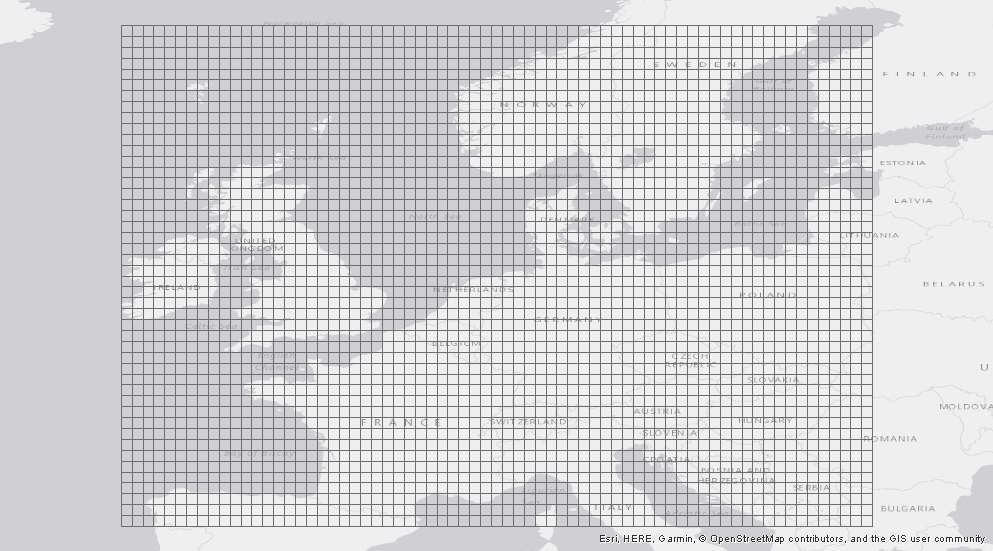
\includegraphics[width=0.9\textwidth]{figures/grid}
\end{center}
  \caption{Map of the grid cells used to abstract the EUROEVOL data set}
  \label{fig:grid}
\end{figure}

The EUROEVOL data set focuses on Neolithic Europe, covering from the late Mesolithic to the Early Bronze Age, as such it is an invaluable source of information about the changes to society taking place during this time. To visually analyse such a large data set, it is necessary to abstract the raw data into a representation that can be manageably displayed at a continental level, while still demonstrating the spread of Neolithic culture and practices. 

\subsubsection{Data Manipulation}
Spatially this can be accomplished by going from a point based representation, to a cell based, while this will loose the accuracy of point data, it will also reduce the clutter of spatial clusters of points. By providing a single value for each cell they are kept consistent, removing the disparity caused by intensive investigation in some areas, and lack of investigation in other areas. The grid used for this analysis is shown overlain on a modern map of Europe in figure~\ref{fig:grid}. From a temporal perspective the abstraction can be done by giving each cell a single date value. In order to model the spread of the Neolithic, the earliest date is used as the process under investigation is inherently concerned with the earliest record of the Neolithic in any particular region. As the date values are radiocarbon dates and are therefore probability distributions the mean value is taken from the calibrated distribution. The data set requires processing to perform this transformation, the steps taken are as follows:
\begin{enumerate}
\item Dates are loaded into OxCal and then calibrated
\item Calibrated means are extracted using \citet{doug_cowie_2018_1297321} into two csv files
\item The CommonSites table from \citet{Manning:2016fk} is updated to include its grid cell number, using ArcGIS
\item CommonDates, CommonSites and means tables are linked to generate an output table that contains date ID, mean value and cell ID
\item The earliest Neolithic date for each cell is extracted using \citet{doug_cowie_2018_1297321}  and written to a csv file
\end{enumerate}

\subsubsection{Broad Trends}
\begin{figure}
\begin{center}
	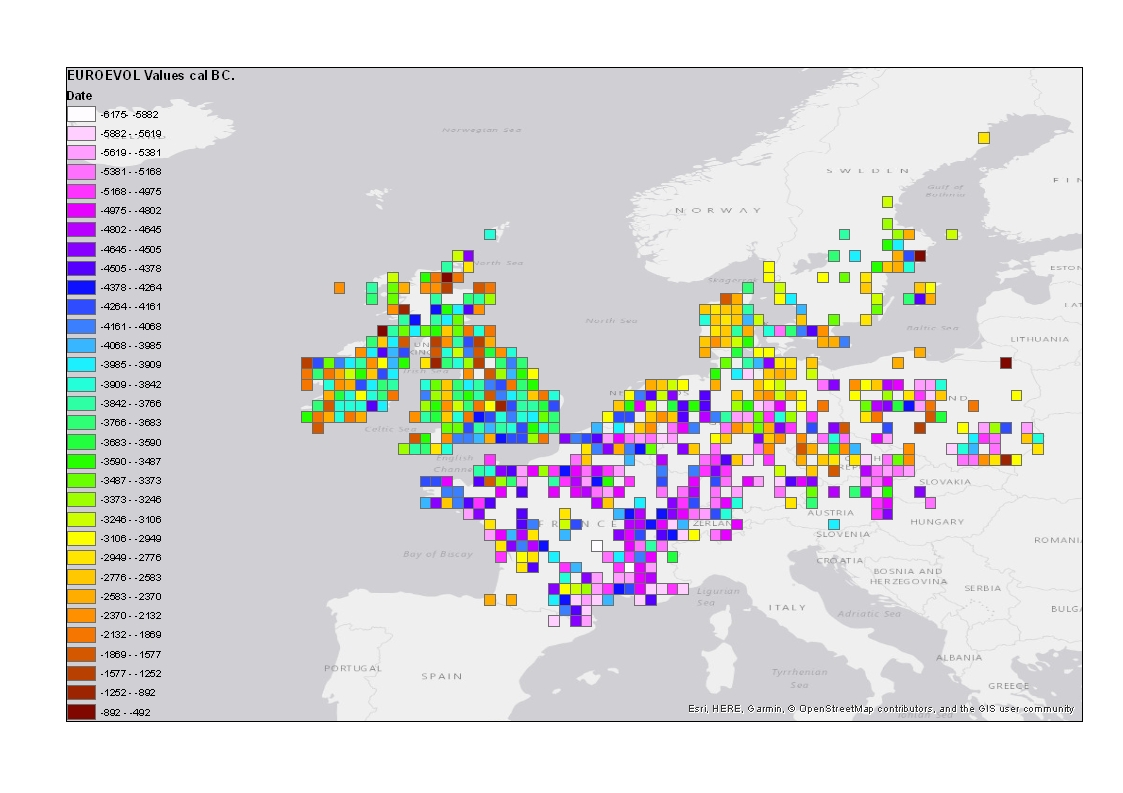
\includegraphics[width=0.9\textwidth]{figures/euroevol-detailed3}
\end{center}
  \caption{Map of first Neolithic dates from EUROEVOL data set, dates are classified using the geometric interval of the mean date values}
  \label{fig:euroevol-detailed1}
\end{figure}

The results of an initial display of this data, using the geometric interval of the mean dates is shown in figure~\ref{fig:euroevol-detailed1}. This shows a trend in the data (which must not be over relied up as the output is based entirely on means of radiocarbon dates) as the cell values change from white and light purples across the south of France, up through Switzerland and Germany, where they fan out more thinly across the Czech Republic and Poland. The values move through to dark purples and blues spreading north and west, and then on to greens, most clearly across the British Isles. They then turn through the yellows to oranges around the north and north-western edges of the data set, clearly going up through Germany and into Denmark. The same broad trends are shown more clearly when the date values used to define the different colours are rationalised upon arbitrary interval, as in figure~\ref{fig:euroevol-detailed2}. Here the time intervals around the middle of the range, from 4700 cal B.C. to 3000 cal B.C. are shown at 100 year time steps, with the preceding time steps having broad, 200 year time steps and the time following 3000 B.C. being grouped very broadly into three steps. 

\begin{figure}
\begin{center}
	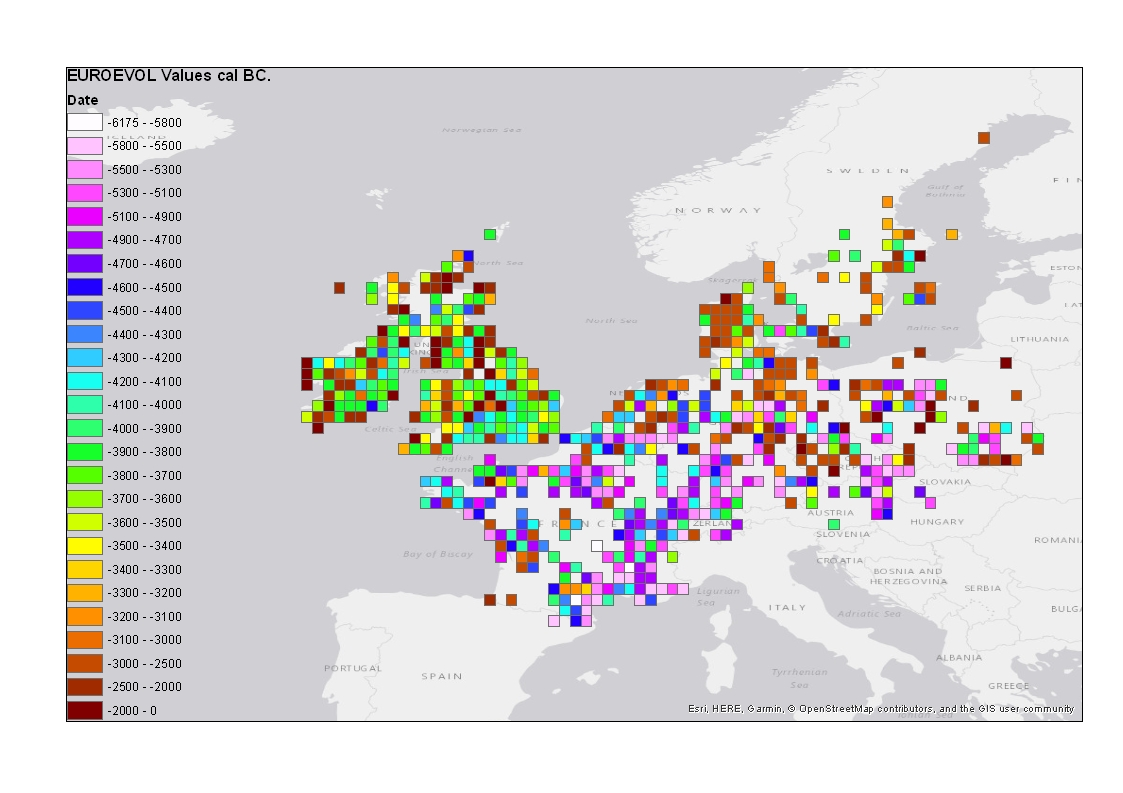
\includegraphics[width=0.9\textwidth]{figures/euroevol-detailed2}
\end{center}
  \caption{Map of first Neolithic dates from EUROEVOL data set, dates are classified using an arbitrary interval with additional intervals in the range 4700 B.C. to 3000 B.C. }
  \label{fig:euroevol-detailed2}
\end{figure}

\subsubsection{Gaps in the Data}
As well as the broad trends of the spread of the Neolithic, the tail of this data set is also particularly interesting, the broad groupings of values from 3000 B.C., in particular 2000 B.C. onwards we might expect to be applied to very few cells across mainland western Europe and the British Isles, as by this time the Neolithic was already well established. There are a significant number of post 2000 B.C. cells across Britain which presumably come from the sparsity of the data set. This is potentially an interesting finding with respect to the SPD approach, as these cells likely represent areas where the Neolithic was already established, but that we simply don't have any radiocarbon dates for until much later. Any population counts are then clearly lacking in data from these cells, where it is likely Neolithic populations existed much earlier than 2000 B.C. These results may also be caused by radiocarbon dates with large distributions, whose average value is much later than the start value of the distribution, however it is unlikely that there are so many radiocarbon dates with such wide distributions that they would span more than a few hundred years.

The appearance of later values within areas of much earlier values is spread relatively broadly across the data set. However where the cell colours change every 100 years, such differences are more likely down to the probabilistic nature of radiocarbon dates and the use of a simple mean to represent them. Although some cells are so much later than those around them that this seems unlikely, for example a row of two orange and one yellow to the south of France, and several individual yellow cells in Austria. Again these are potentially gaps in the data, suggesting that the SPD is likely miss-representing earlier Neolithic population levels, and therefore potentially not showing accurate changes.

\begin{figure}
\begin{center}
	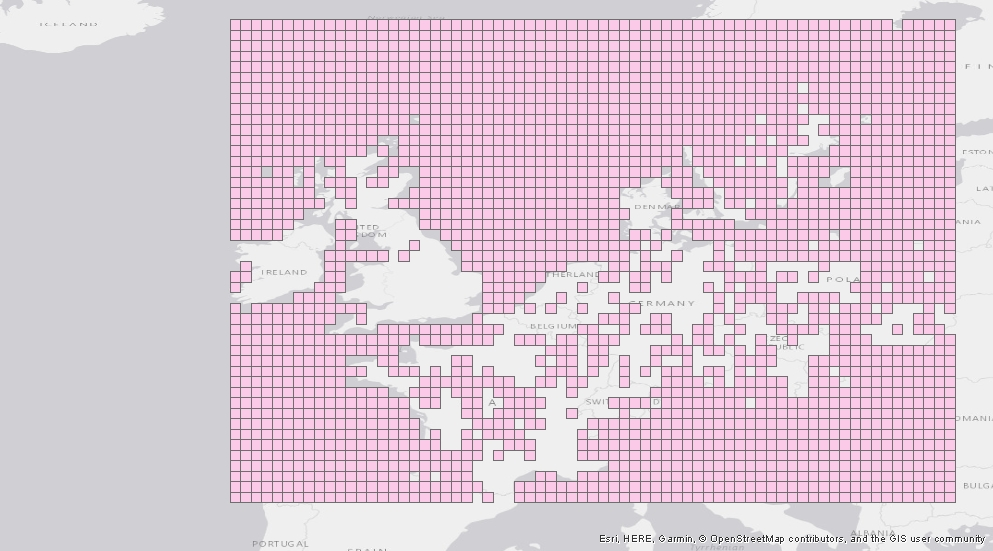
\includegraphics[width=0.9\textwidth]{figures/euroevol-null}
\end{center}
  \caption{Map showing empty cells in the EUROEVOL data set}
  \label{fig:euroevol-empty}
\end{figure}

Figure~\ref{fig:euroevol-empty} shows all the cells for which there is no date categorised as Neolithic in the data set. The vast majority are from areas of sea, or areas outside the study area of the EUROEVOL data set. However there are a surprising concentration across central France, and up into Germany, which makes up a large area for which there are no Neolithic dates. Again, this is a significant omission from the data set, which must impact its ability to represent levels of population during the period. Just as interesting is the presence of data in the outlying regions of the study area, such as Scottish Islands and Sweden (but not Norway) especially Gotland, Aland and to the far north on the top row. These pockets of data suggest there are many gaps in the current record.

\subsubsection{Mesolithic - Neolithic Transition}
\begin{figure}
\begin{center}
	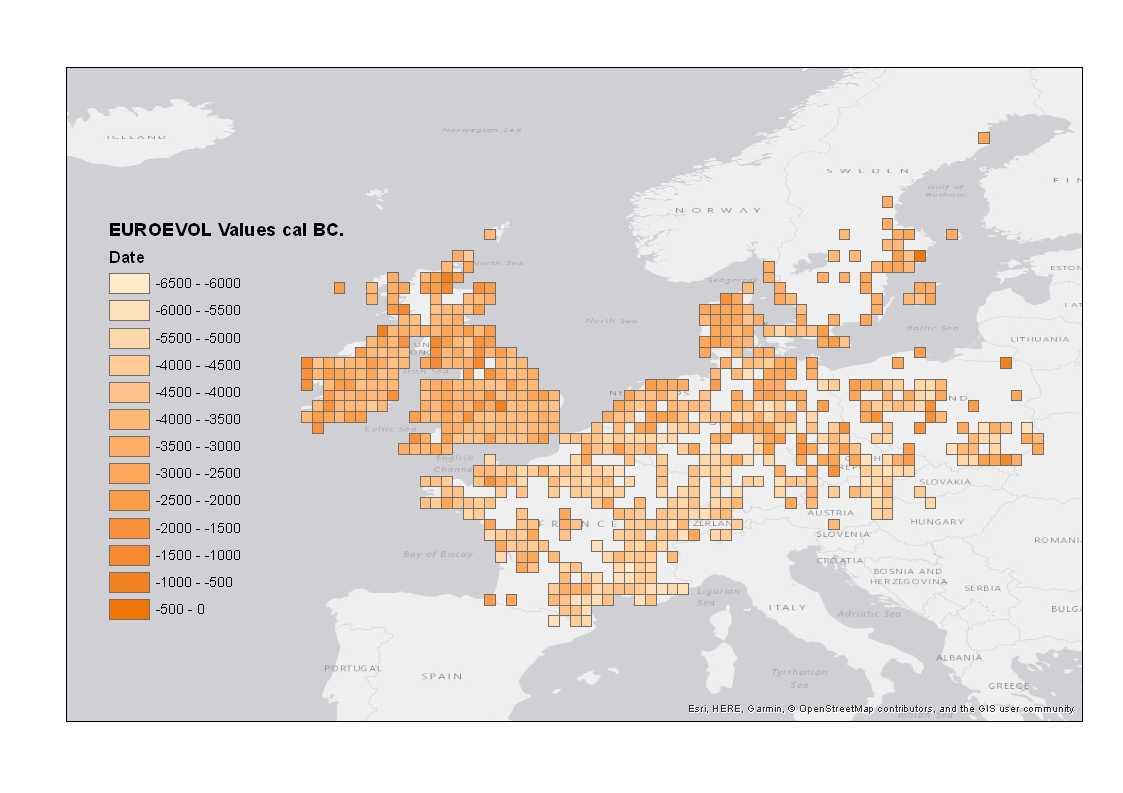
\includegraphics[width=0.9\textwidth]{figures/euroevol-values}
\end{center}
  \caption{Map of first Neolithic dates from EUROEVOL data set, dates are classified using an arbitrary interval of equal duration}
  \label{fig:euroevol-all}
\end{figure}

The data set is presented using a consistent scale in figure~\ref{fig:euroevol-all}, while the trends are less clear that using the convex scale of figure~\ref{fig:euroevol-detailed2} they are still visible in the gradient of the colour of the cells, in particular most of the later outliers still stand out. Using this scale, the cells can be split in half temporally, as shown in figure~\ref{fig:euroevol-laten}. The cells in orange are post 3000 B.C. by which time we might have expected the Neolithic to be established across the entirety of north western Europe, however there are large groupings of such cells, particularly in Britain, also Germany, the low countries and Denmark. It seems unlikely that some parts of these areas (particularly the isolated cells) remained pre-Neolithic for so long. The 500 year intervals makes it less likely that the results are down to taking means from radiocarbon dates, and more likely that it is due to the sparseness of the data set.

\begin{figure}
\begin{center}
	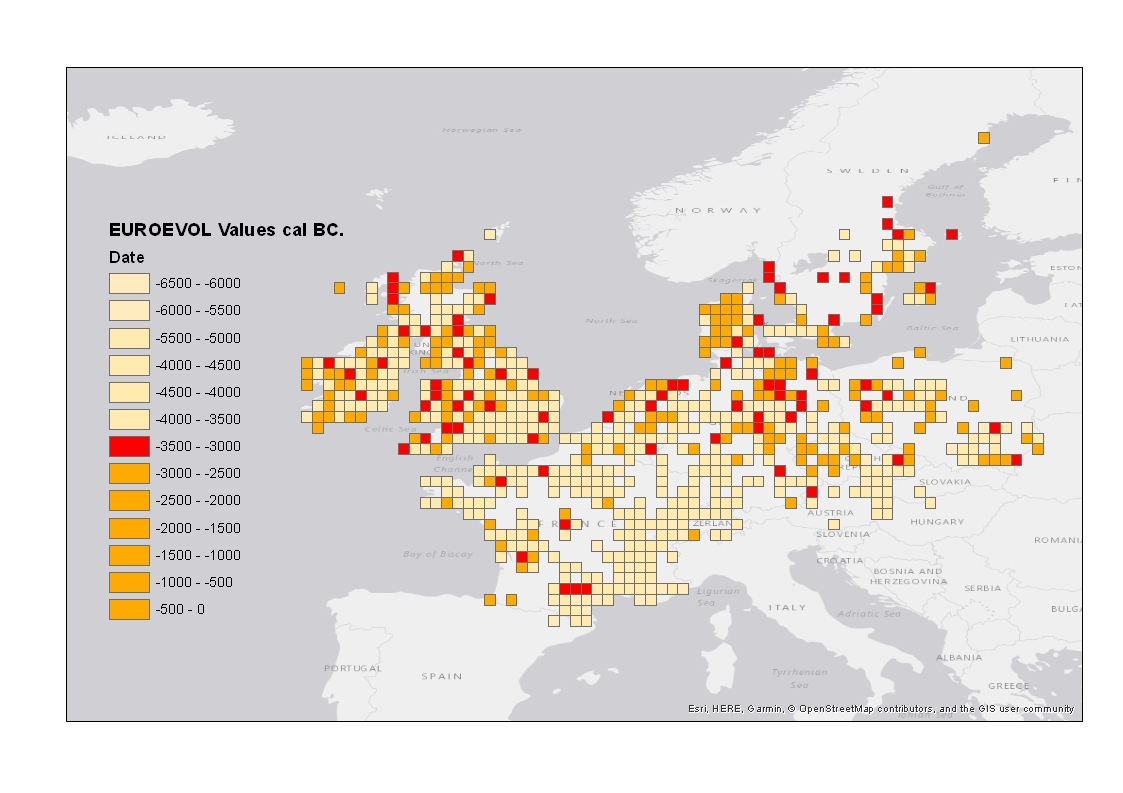
\includegraphics[width=0.9\textwidth]{figures/euroevol-late-neo}
\end{center}
  \caption{Map of first Neolithic dates showing before and after 3000 B.C.}
  \label{fig:euroevol-laten}
\end{figure}

This unapologetically visual EDA has highlighted issues with the data set and has also shown both the potential for EDA as a spatio-temporal technique and for the EUROEVOL data set as a subject of analysis. In order to investigate the data set, in particular how it captures the spread of the Neolithic across space and time, further analysis is required. In this case an appropriate technique would be modelling the underlying data set, as noted it has been the subject to a variety of process. The exact nature of which varies across space and time, so the model should either be extremely detailed, or capable of representing a variety of processes and uncertainties through abstraction.

\subsection{Modelling}
Archaeology has a rich tradition of modelling and simulation, from a variety of epistemological traditions and has been influenced by similar traditions in many other disciplines. The kind of model required to represent the spread of Neolithic dates must be suitable for large scale, stochastic processes. A potential source of inspiration is the field of epidemiology, which has a different, although similarly rich tradition of modelling and simulation. \citet{doi:10.1111/j.1467-9671.2012.01329.x} provides an overview, demonstrating a move from the early forms of classical models, to modern agent based models (among other types). They have focus on the modelling unit, which is similar to the concept of resolution above, in that models focused on the individual would be expected to have a greater resolution than those focused on the sub-population, and they will be greater still than those focused on the population. However models with a greater modelling unit can still model at a high resolution, by explicitly modelling a large proportion of the processes that have been identified to have contributed to the archaeological record. A clear difference between the two traditions is the objectives, while epidemiological models are often used to predict the behaviour of a new outbreak, archaeological models typically focus on hypothesis generation and testing. The data sets are likely to contain similar characteristics, depending on the data used, for example any self-reported data will clearly be biased, data may be fragmentary, especially historical data, or data from countries that do not have the facilities for large scale data gathering and storage. Fundamentally this is a problem of differential reporting, which is analogous to the issue of the data set not being a statistical sample. There is also the potential for the design of the research programme to introduce biases, for example focusing on specific sub-populations will likely lead to an over-representation. Crucially is the similarity that both attempt to model processes that contain a spatial and a temporal component. In order to determine what can be adapted from epidemiological modelling, it is important to consider the fundamental nature of what is being simulated. Communicable diseases are those which are transmitted from individual to individual and if enough people become infected can spread at scale, as an epidemic. Such models typically use a finite set of states to model infection status, with the archetypal set being the SIR (susceptible, infected, recovered) model. The specific mechanics of the model dictate how the model unit changes state, in an attempt to replicate the spread of disease between these units. Clearly any attempt to take an epidemiology model wholesale would require interpreting in the context of the archaeological evidence, and the specific questions being considered.

\subsubsection{Similarities and Differences to Epidemiological Models}
For the purpose of modelling, analogies can be drawn between the spread of culture and the spread of disease. Both are transmitted either person to person or by the movement of people, yet have observable effects at the population level. Both describe changes moving across a population and both can be modelled as the state of a unit of population, from individual up to a whole society. Yet the underlying phenomenon are clearly different, the spread of a pathogen compared to the transfer of culture and knowledge. Not only this, the timescales involved are also very different, with the spread of the Neolithic taking thousands of years, a much larger time scale than any epidemic. Likewise the effects are clearly different, while infection by a disease may cause ill health, or even death, the transition to agriculture shifts subsistence patterns and the introduction of ceramics creates a new medium of material culture. However equivalence is not a necessary condition for an analogy, the analogy holds on the basis of the similarities of the processes, as constructed for the simulation. The broad brush strokes (or low resolution) used by some epidemiological models, focussing exclusively on the pattern of spread, are therefore a much closer fit to the spread of culture than very detailed models. That such models can benefit the study of epidemiology and predict health outcomes \citep[4]{doi:10.1111/j.1467-9671.2012.01329.x} (despite the lack of detail) suggests that they may provide corresponding value to our understanding of the spread of the Neolithic.

\citet{doi:10.1111/j.1467-9671.2012.01329.x} categorises a set of spatially oriented models, based on modelling unit and mobility. Individual-based cellular automata provide a compromise between modelling unit, mobility and model complexity, crucially they model the interactions between units \citep[e.g.][]{WHITE2007193,FUENTES1999471,Yang:2017fk}. This level of detail enables a simulation that does not spread homogeneously across a population (as for example wave based population models would do) and can also facilitate long distance transmission via ``leapfrogging'' \citep[6]{doi:10.1111/j.1467-9671.2012.01329.x}. The local transmission of disease is controlled using rules that determine how the disease is spread from cell to cell, the cells are generally assumed to be immobile and may be heterogenous in nature. While other types of models could be used instead, in particular individual based or mobile population models, as mentioned above there is a danger of over-fitting with more detailed model types. The problem of attempting to replicate too many processes, in too much detail, so the exercise becomes one of determining a set of parameters for the processes that simply fit the data. For data with potentially unknown biases and many different model configurations can make it difficult to draw any solid conclusions from the exercise.

\subsubsection{Applying an Epidemiological Model to Archaeological Processes}
To apply an epidemiological model to the spread of the Neolithic requires a re-consideration of a few key points, firstly the different states that can be assigned to units of population, also how the method of transmission is encapsulated in the model, and what the unit of study is. In individual focused epidemiological models, the unit of study is clearly an individual person, this inherently requires a degree of information about the population size, which is clearly problematic for the period under study. Of course epidemiology also studies the spread of disease between animals and plant life, in fact, due to the assumption that the unit under study is immobile for cellular-automata this type of model is typically used for studying disease in plants \citep[6]{doi:10.1111/j.1467-9671.2012.01329.x} although not exclusively \citep[e.g.][]{Yang:2017fk}. For the spread of the Neolithic, taking the individual as the unit of study might seem obvious, but as mentioned there are some large gaps in the data around populations. Also at the individual level there are gaps in our knowledge of small scale processes, such as how hunter-gatherers and farmers interacted and of those local scale processes that caused the Neolithic culture and practices to spread. However there is clear evidence that they did spread, at a continental scale there is significant amounts of evidence. In order to model this spread, it is perhaps more appropriate to think of a geographic area as the individual, with ``infection'' occurring at the date for the earliest evidence for Neolithic practices or culture in that area. To continuing on from the EDA above by using each grid cell as the individual. Taking spatial area as the individual means that the immobility assumption of cellular automata does not undermine the choice of model for the problem. It also means that the process of transmission can be considered relatively broadly, not from person to person, but between distinct spatial areas. With this in mind, the set of states for each location is only `Susceptible' and `Infected' (to retain the epidemiological terms) if we assume that once the Neolithic has spread to an area, its inhabitants do not revert to their previous way of life (at least not entirely) and that some components of the Neolithic toolkit are retained, enough for archaeologists to classify it as Neolithic. The EUROEVOL dataset is a clear candidate for investigation by modelling and cellular automata is a good fit to model the creation of the data set.

\subsection{Using Cellular Automata with the EUROEVOL dataset}
A custom modelling tool \citep{doug_cowie_2018_1297319} has been designed to demonstrate the applicability of this type of model to the dataset. It provides only the basic modelling facilities required to explore the distribution of data. 

\subsubsection{Description of the Model}
The model generates a csv output for first Neolithic dates for each grid cell. The algorithm generates a grid world, and then performs a specific number of model steps, where each step determines how the Neolithic has transmitted during that step, any cells that it spreads to take the number of that turn. After all the steps have run, the resultant grid is output. The algorithm is modelled on an SIR type model, although as described above it only contains two states, susceptible and infected.

The transmission process can be modelled as two distinct subprocesses, the direct spread between cells and the indirect ``leapfrogging''. In order to make these non-deterministic, a stochastic model is employed, which will also create an element of uncertainty to accommodate for the issues with the data set. This is important as with the data set available it is unlikely to be possible to match a simulation to the data perfectly, and even if we did, the addition of new data could render a deterministic model obsolete if the new data does not fit the model. While a stochastic processes is unlikely to generate data matching the observed data set and will generate slightly different data with each run, the uncertainty introduced will make the model a closer approximation to the underlying processes.

Direct transmission is modelled as the probability that a cell infects one if its direct neighbours, these being the eight cells that surround it, or Moore neighbourhood. If we assume that a cell could potentially infect multiple neighbours (or none) then the stochastic process for this is based on the probability of infection for each neighbourhood cell. Indirect transmission is considered from the perspective of the cell that might be infected, it is essentially the probability that infection spreads from an extended neighbourhood. The greater the number and the closer proximity of infected neighbours, the greater the chance of infection. 

\subsubsection{Replicating the EUROEVOL Dataset}
In order to attempt to replicate figure~\ref{fig:euroevol-all} the model will be designed to run for ten steps and also feature a seeding stage, which will take the values for the first two sets of dates from the EDA analysis above. These are the sets of values falling into date ranges from 6500 B.C. to and 6000 B.C. and 6000 B.C. to 5500 B.C. (both are used as the first set only contains a single cell). In order to fully implement the algorithm, it is necessary to determine key parameters from the original data set, specifically, the rate or probability of direct and indirect transmission. The published values in \citet{doug_cowie_2018_1297319} were identified via a process of manual inspection and experimentation. A more robust method was not used due to the vagaries of the original data set, it's biases and the use of means to represent dates. As such any model derived from this data should also be treated as an approximation and an experiment.

\begin{figure}
\begin{center}
	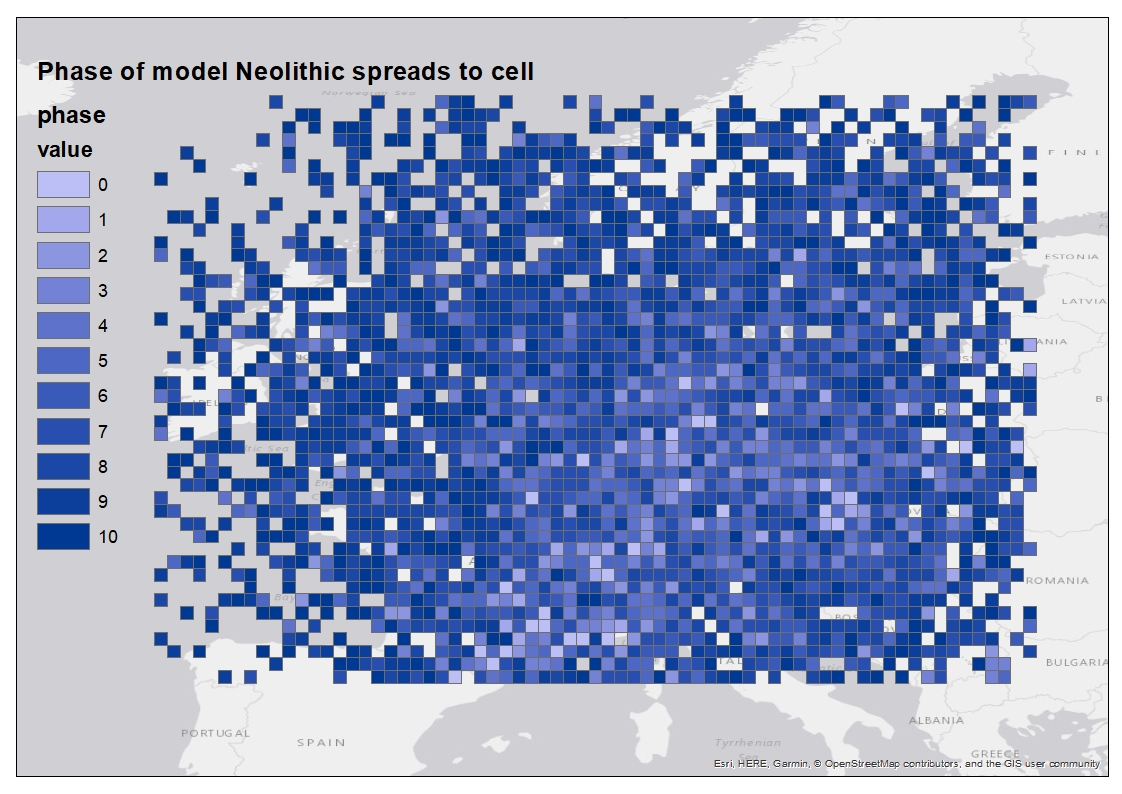
\includegraphics[width=0.9\textwidth]{figures/model-all}
\end{center}
  \caption{Map of all values from generated data set}
  \label{fig:model-all}
\end{figure}

A data set generated by a single run of the model has been plotted in the same way as the original data set. Figure~\ref{fig:model-all} is the counterpart to figure~\ref{fig:euroevol-all}, showing some clear differences. Most obviously the model is running on a plain grid, so does not respect geographic features, such as the sea. There is also the potential that geographic features could act to slow down the spread of the Neolithic, although over the modelled 500 year time steps, it is unlikely this would be particularly visible. Also of note is that the model has spread in all directions, where as the original data set is more directed, this is in part due to the original data set being collected based on modern boundaries, for example Spain, Italy and the Balkans are excluded. It has also reached further, to the north of Norway and Sweden, where there is very little data in the original data set. 

\subsubsection{Gaps in the Data}
\begin{figure}
\begin{center}
	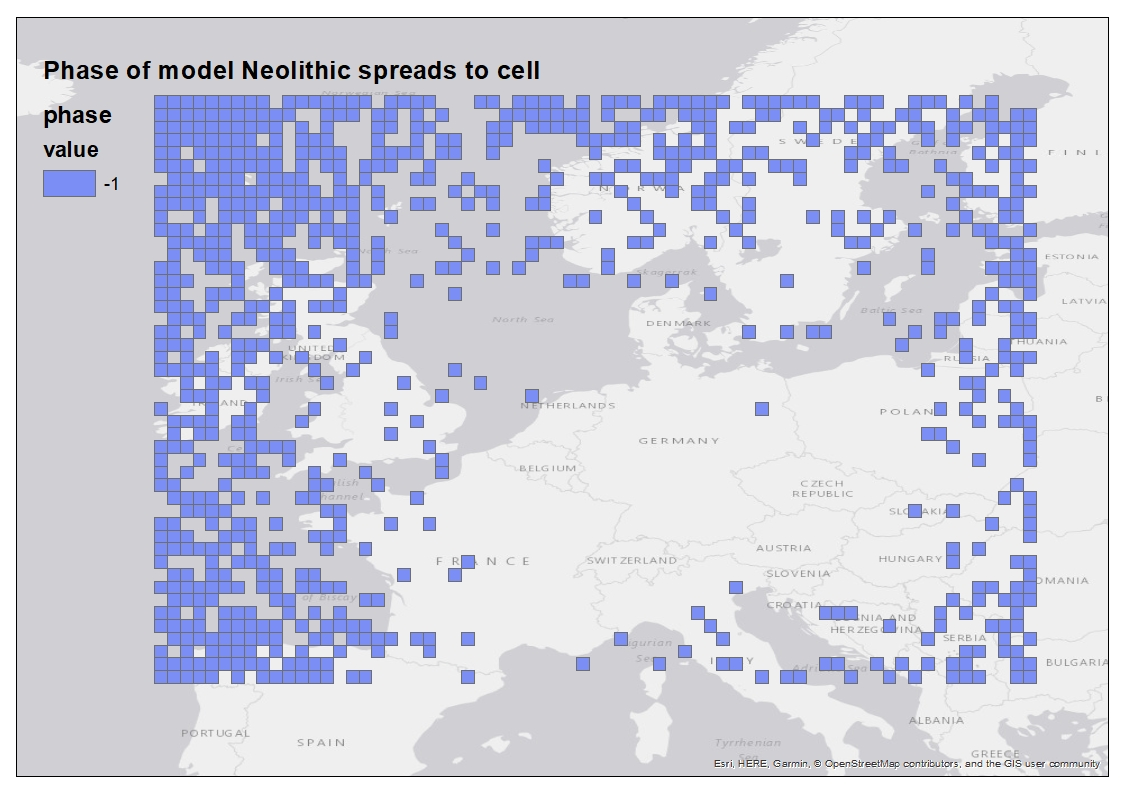
\includegraphics[width=0.9\textwidth]{figures/model-empty}
\end{center}
  \caption{Map of empty cells from the generated data set}
  \label{fig:model-empty}
\end{figure}

As with the true data set there are cells that have no value, these are shown in figure~\ref{fig:model-empty}. These cells tend be around the periphery, or sea. There are some cells in France and Britain, but the distribution is clearly focused towards the edges of the data set, which is not unexpected - unlike the empty cells from the original data set, which was surprising that there were so many in mainland Europe. This shows that the model process provides an approximation in terms of empty cells, although it is not an exact match.

\subsubsection{Comparing the Generated Dataset to the Archaeological Evidence}
\begin{figure}
\centering
	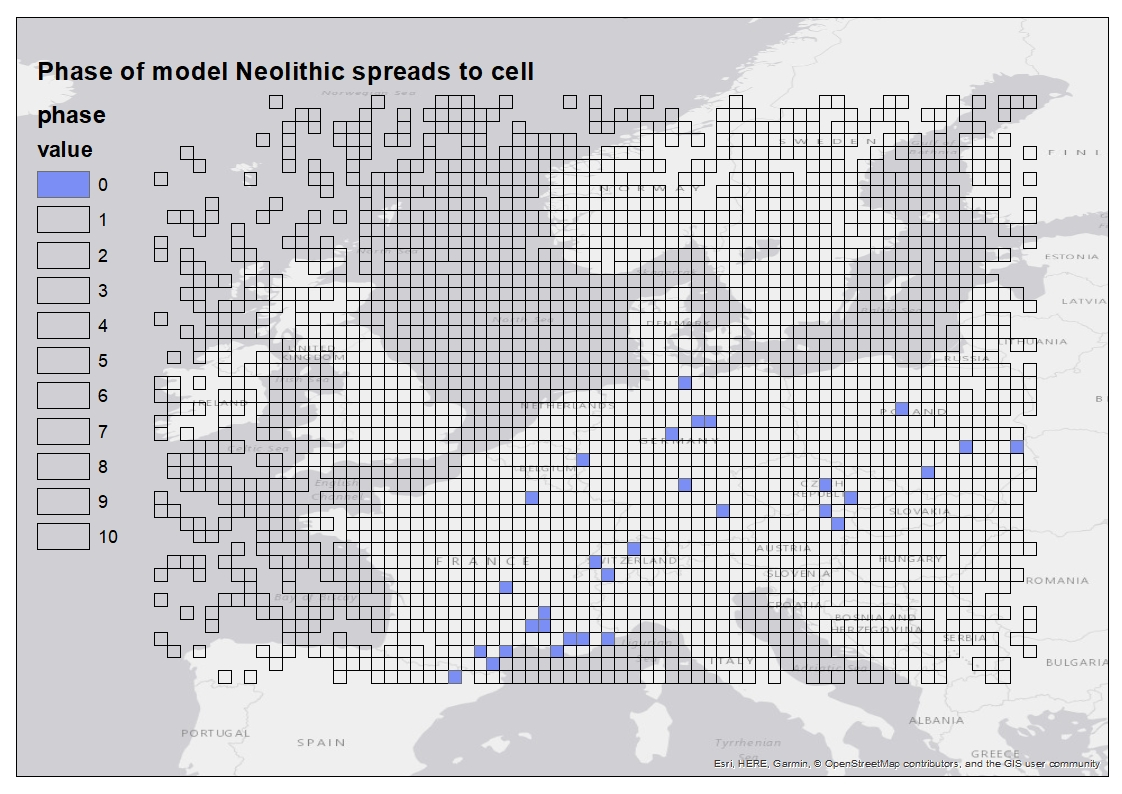
\includegraphics[width=0.8\textwidth]{figures/model-0}
	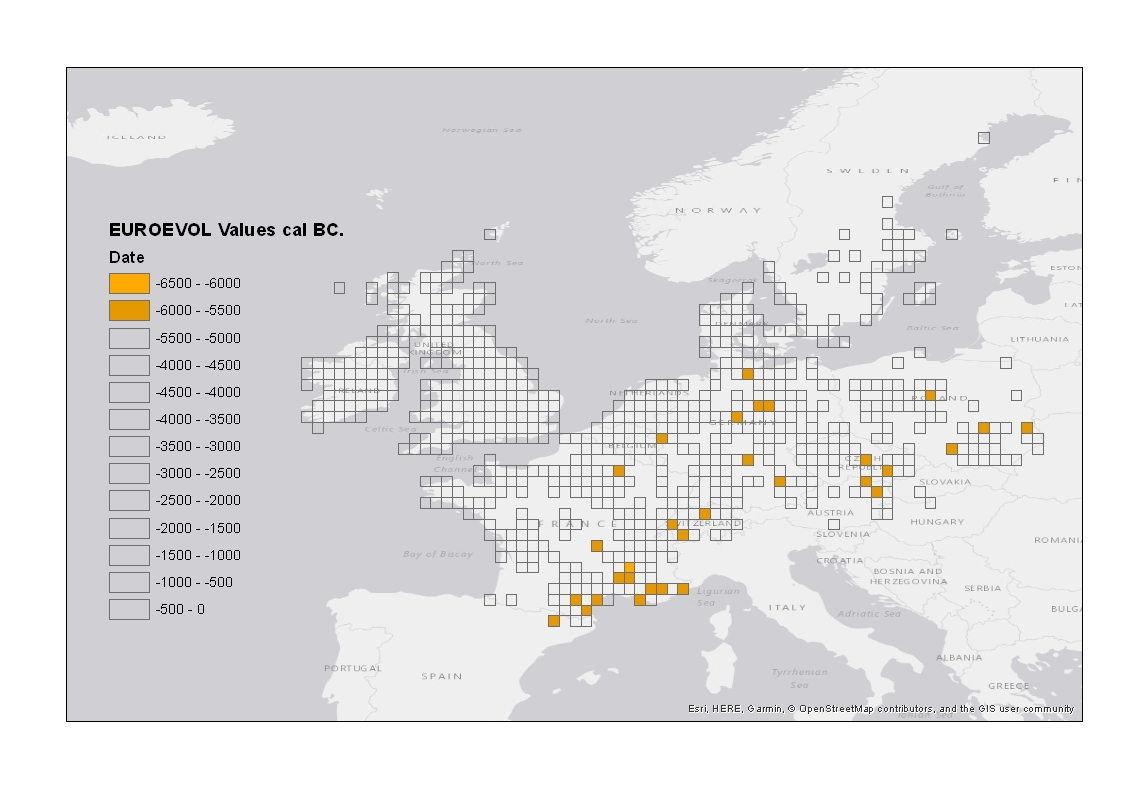
\includegraphics[width=0.8\textwidth]{figures/euroevol-0}
  \caption{Initial model state and corresponding EUROEVOL data}
  \label{fig:compare0}
\end{figure}

Figure~\ref{fig:compare0} shows the initial state of the model and the corresponding two sets of dates from the archaeological dataset. It demonstrates that the model takes the cells from these two sets as its starting state.

\begin{figure}
\centering
	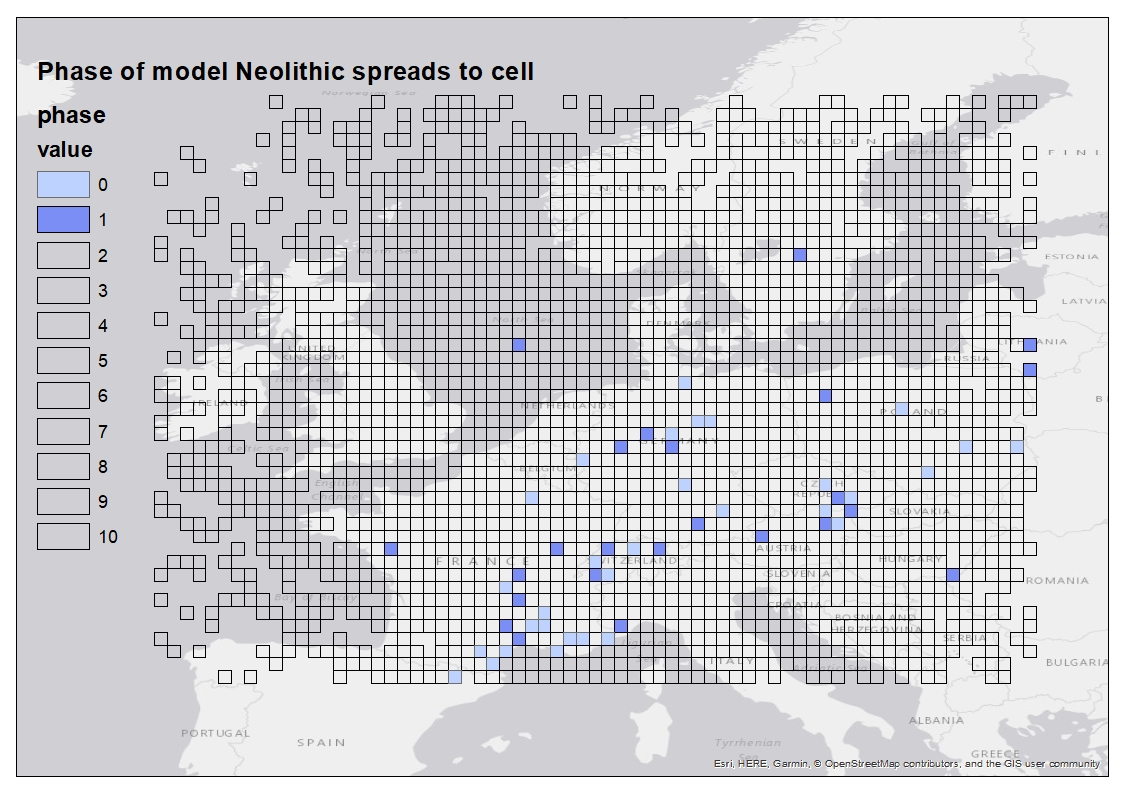
\includegraphics[width=0.8\textwidth]{figures/model-1}
	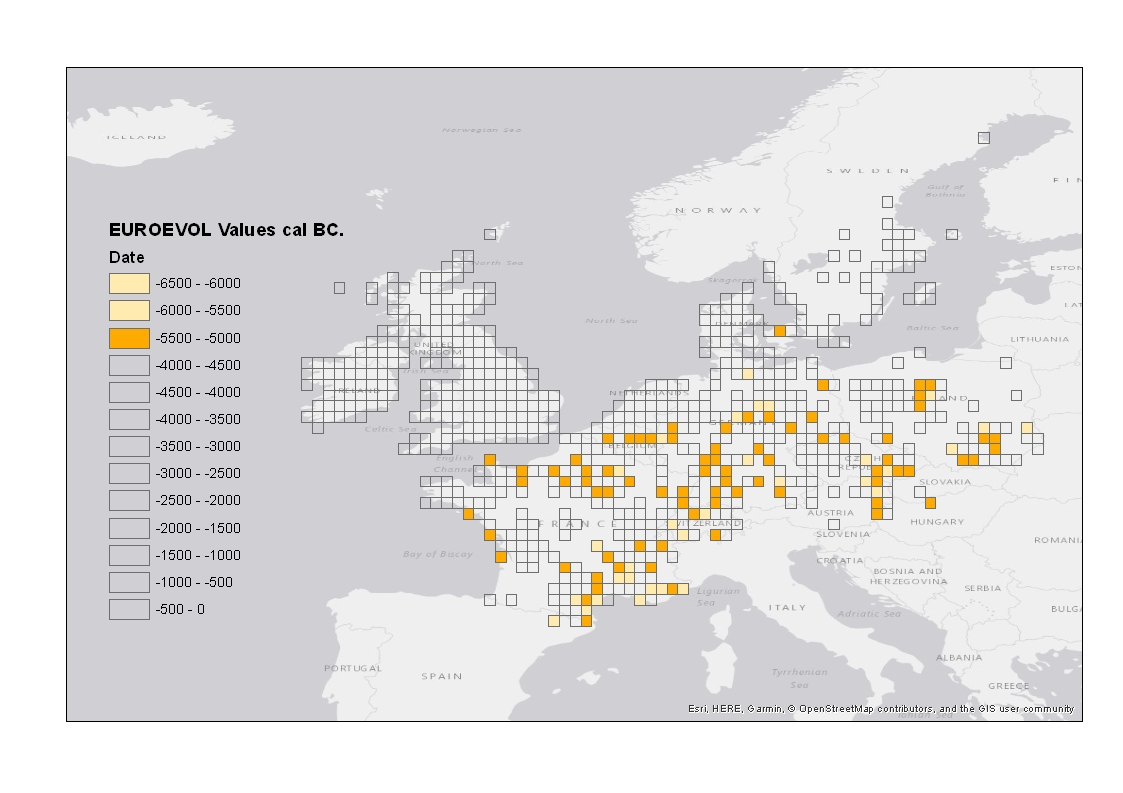
\includegraphics[width=0.8\textwidth]{figures/euroevol-1}
  \caption{Model state after phase one and corresponding EUROEVOL data}
  \label{fig:compare1}
\end{figure}

Figure~\ref{fig:compare1} shows the cells that have become Neolithic after the first step of the model, and the cells that were previously Neolithic, along with the corresponding sets of dates from the dataset. The model has fewer values than the dataset, and these values are distributed over a larger spatial extent, while the dataset values are more concentrated in central Europe, the model values are more focused around those areas that had initial values.

\begin{figure}
\centering
	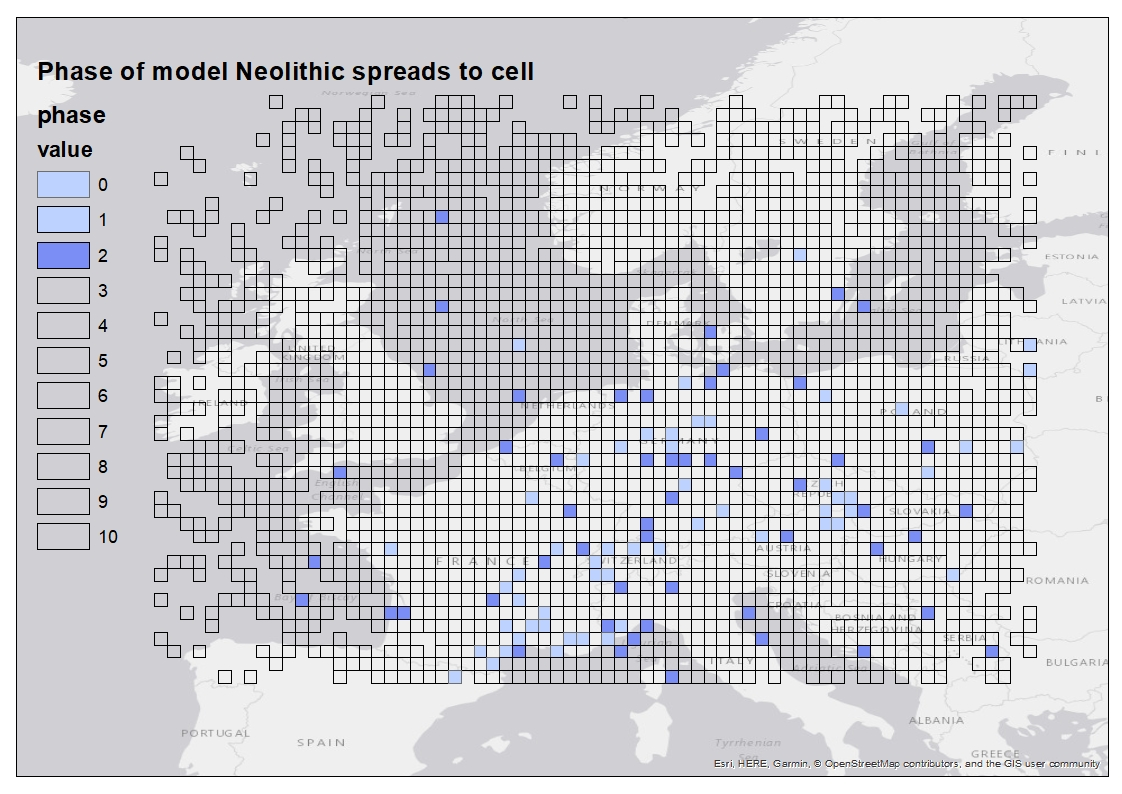
\includegraphics[width=0.8\textwidth]{figures/model-2}
	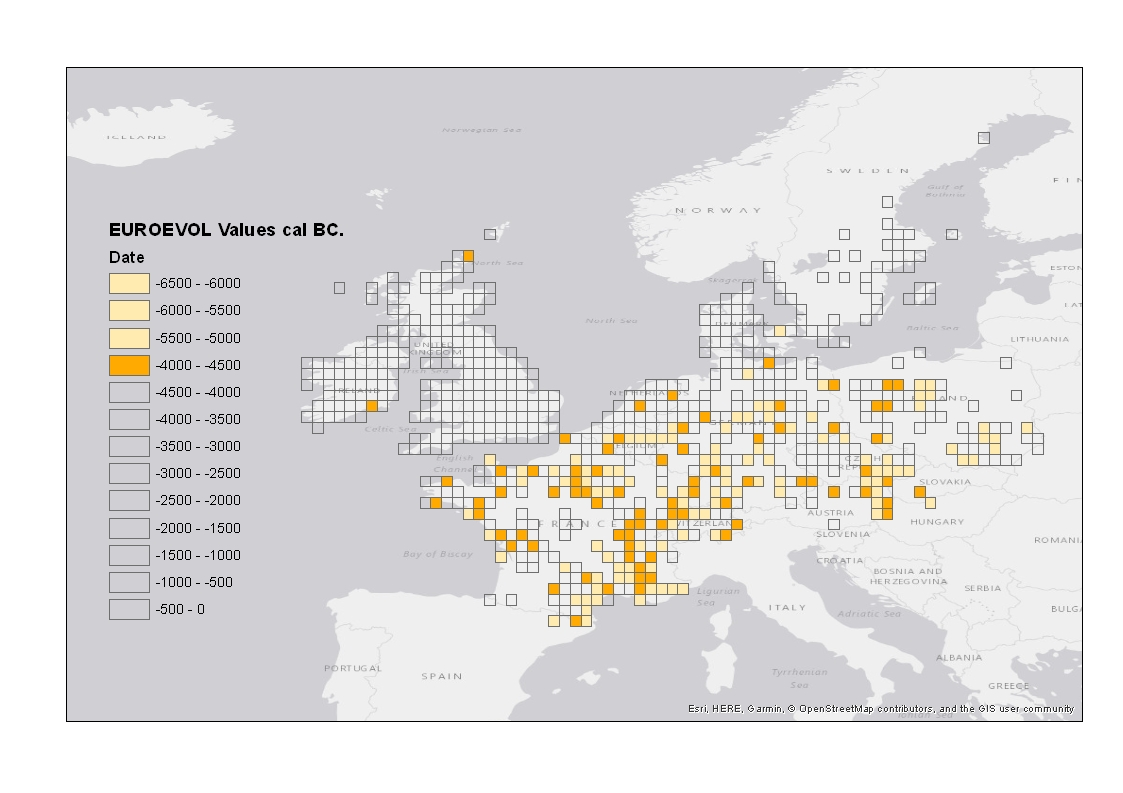
\includegraphics[width=0.8\textwidth]{figures/euroevol-2}
  \caption{Model state after phase two and corresponding EUROEVOL data}
  \label{fig:compare2}
\end{figure}

\begin{figure}
\centering
	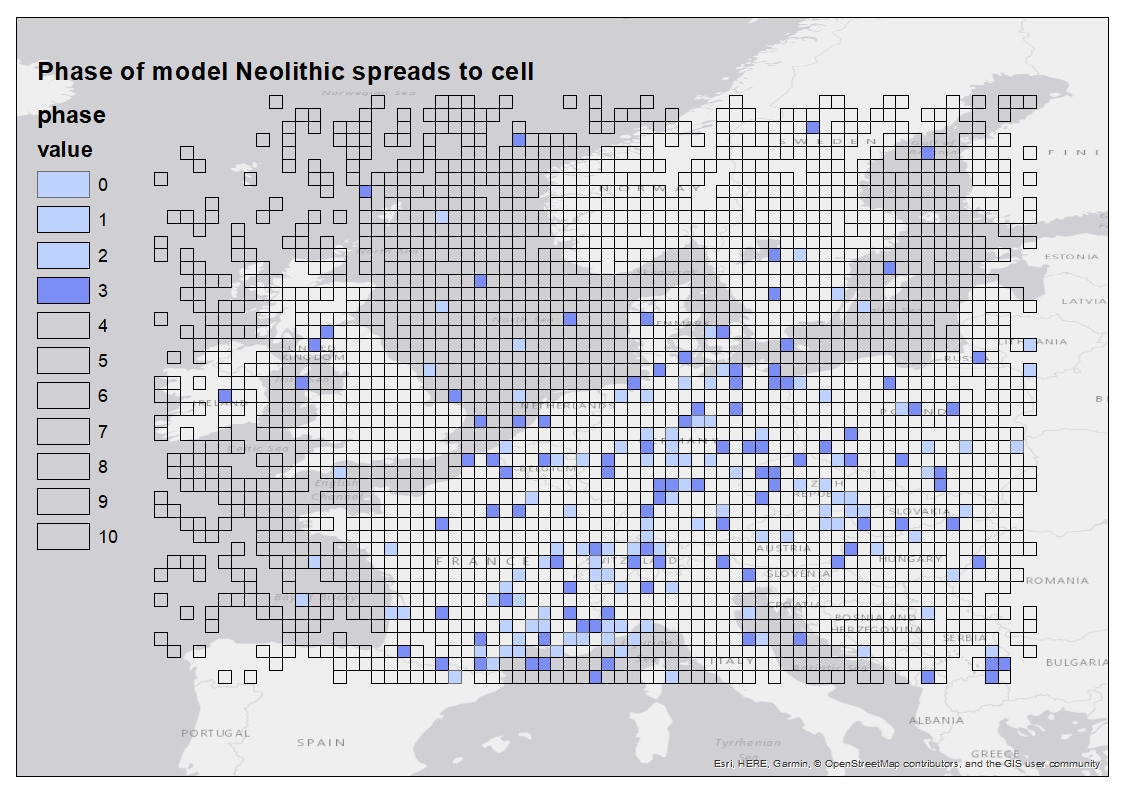
\includegraphics[width=0.8\textwidth]{figures/model-3}
	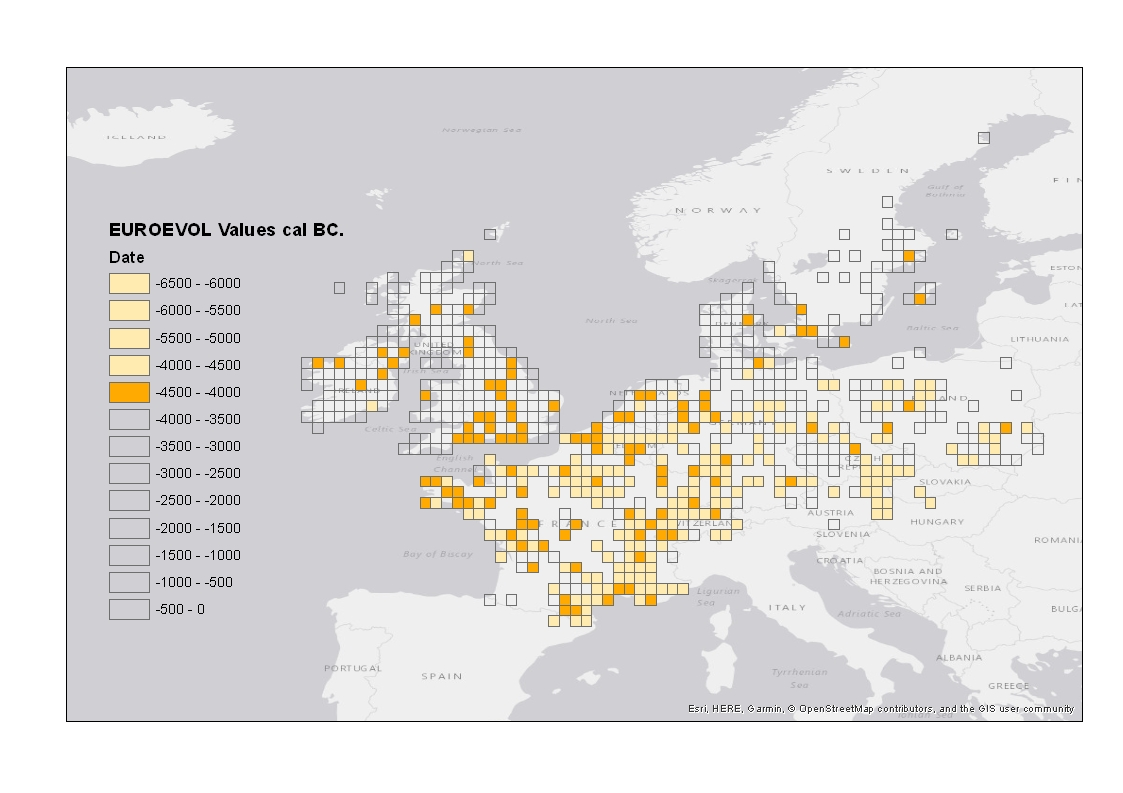
\includegraphics[width=0.8\textwidth]{figures/euroevol-3}
  \caption{Model state after phase three and corresponding EUROEVOL data}
  \label{fig:compare3}
\end{figure}

Figures~\ref{fig:compare2},\ref{fig:compare3},\ref{fig:compare4},\ref{fig:compare5},\ref{fig:compare6},\ref{fig:compare7},\ref{fig:compare8},\ref{fig:compare9} and \ref{fig:compare10} show the progression of the model and the corresponding sets of dates from the dataset. As the model progresses the cells become distributed across a greater spatial extent more quickly and do not conform to geographic boundaries. The model provides a reasonable approximation to the data set across the south of France, up through Switzerland and Germany, to Denmark and then across Poland, up to figure~\ref{fig:compare4}, at which point the model populates more cells on mainland Europe, (with the exception of north-western France) but considerably fewer in Britain. This pattern continues for the remaining steps of the model, although from figure~\ref{fig:compare6} it increasingly deviates as the model spreads out more evenly, and picks up it's pace, where as the original data set slows down, into a pattern more like the infilling of cells. By the final phase,  figure~\ref{fig:compare10}, (which is in fact two sets of cells from the original data set, due to the low number of new cells at this stage) the main differences between the two are, firstly, the gaps in the original data set across France and up through Germany and into Poland. These areas are very close to those that seeded the model and so have been fully populated in the model and secondly, the gaps the model output in northern France and Britain. In addition there are other differences already mentioned, such as where the model has generated data outside of the study area.

\begin{figure}
\centering
	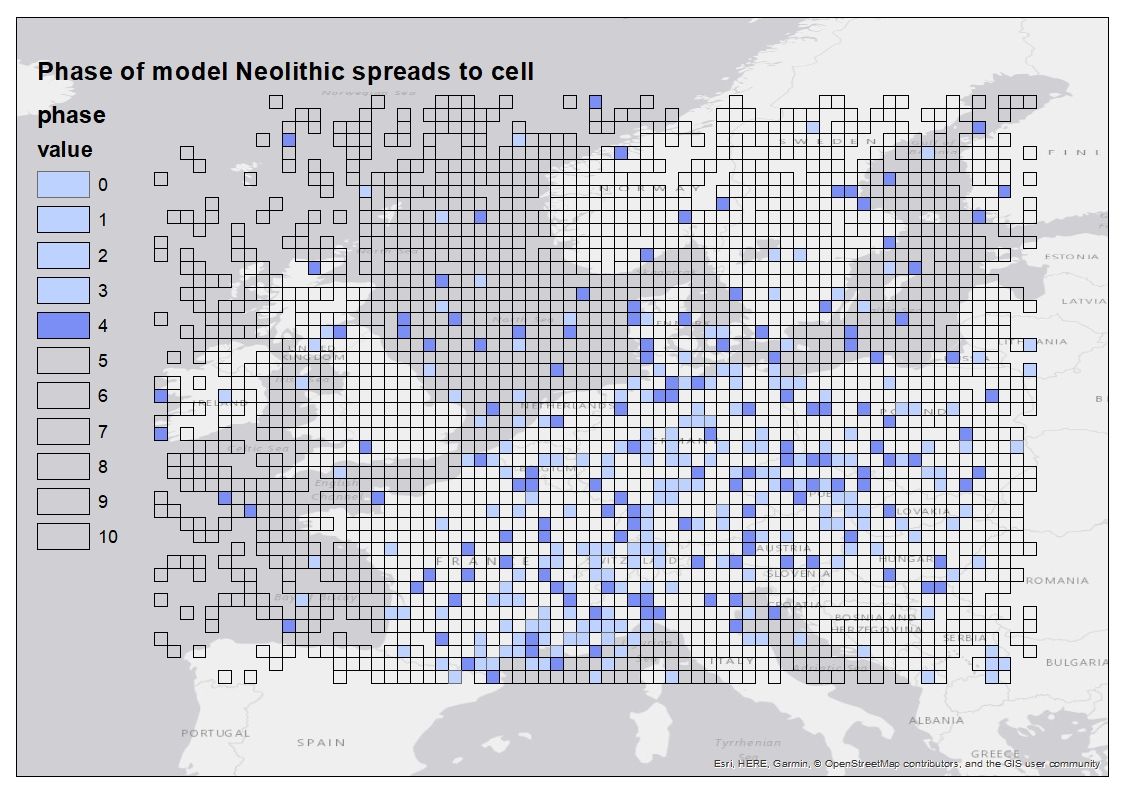
\includegraphics[width=0.8\textwidth]{figures/model-4}
	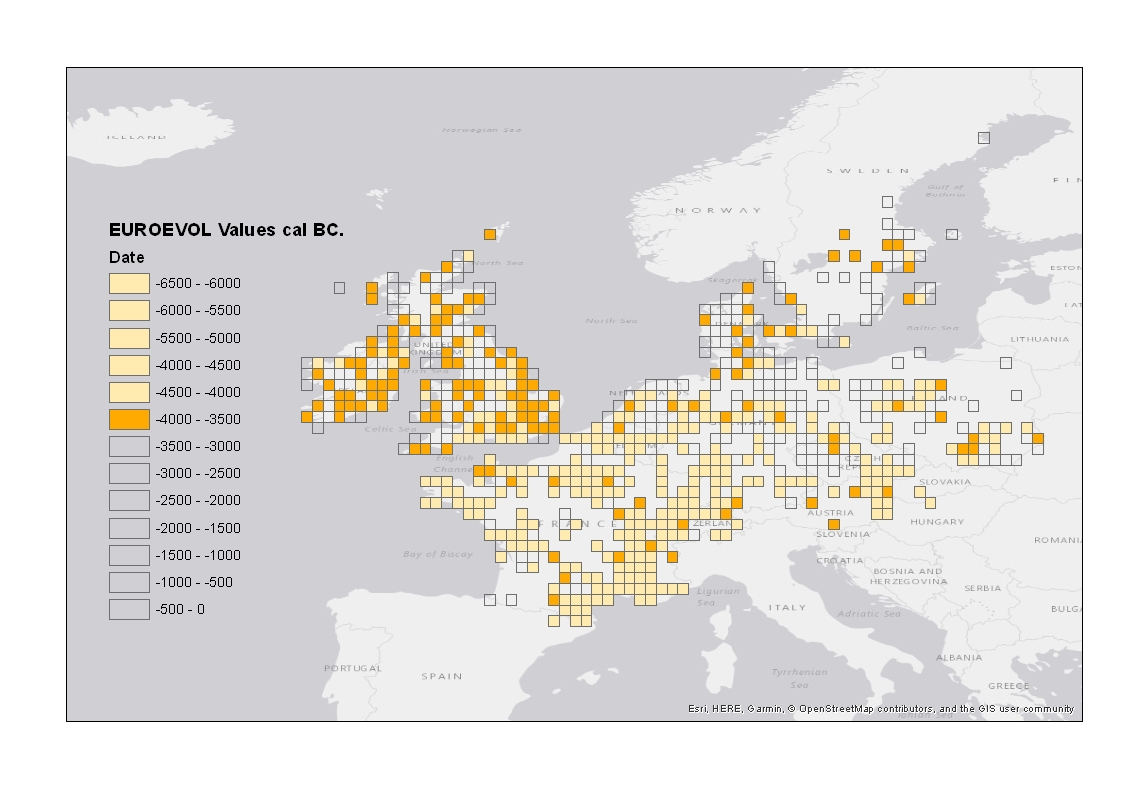
\includegraphics[width=0.8\textwidth]{figures/euroevol-4}
  \caption{Model state after phase four and corresponding EUROEVOL data}
  \label{fig:compare4}
\end{figure}

\begin{figure}
\centering
	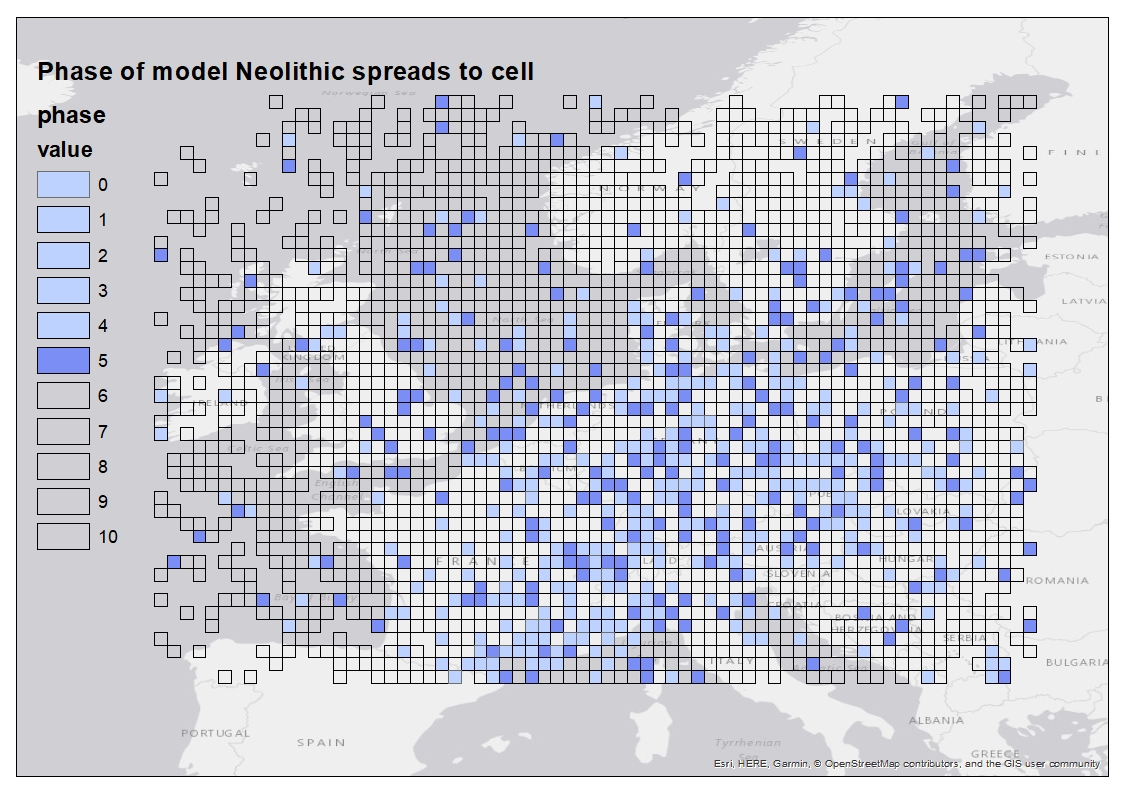
\includegraphics[width=0.8\textwidth]{figures/model-5}
	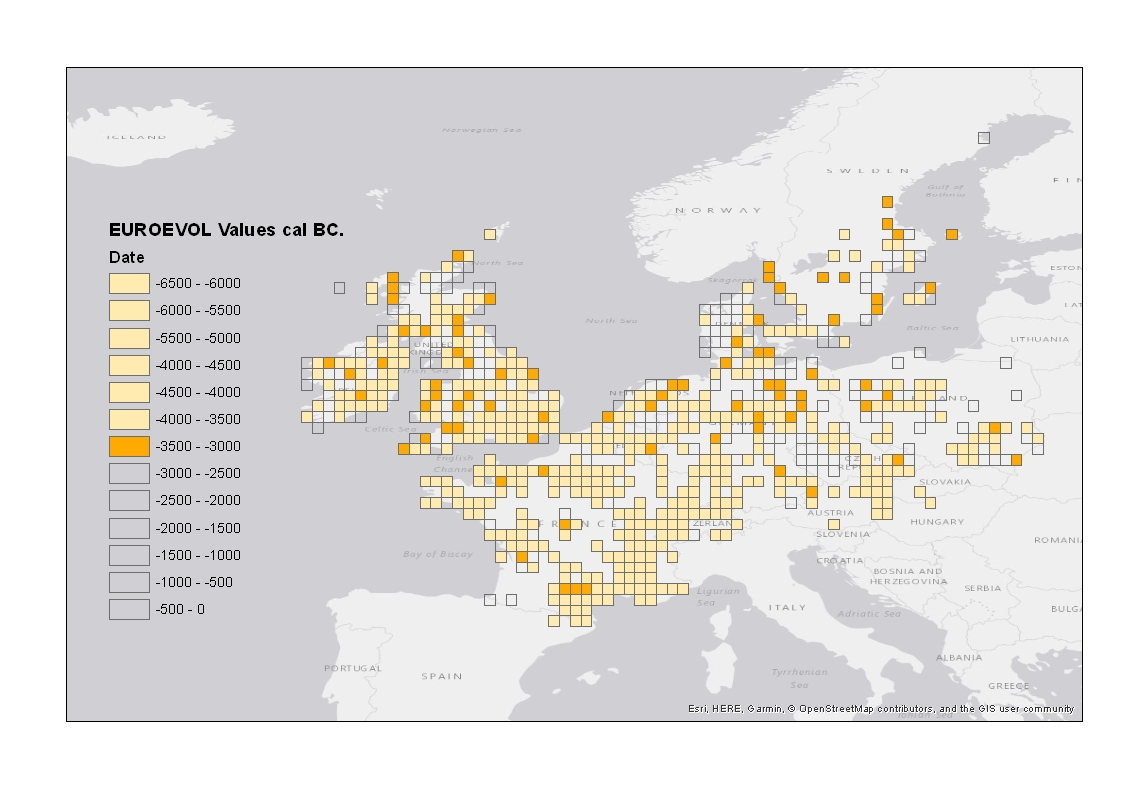
\includegraphics[width=0.8\textwidth]{figures/euroevol-5}
  \caption{Model state after phase five and corresponding EUROEVOL data}
  \label{fig:compare5}
\end{figure}

This leads on to the question of what can such a relatively simplistic model tell us, this can be split into two categories. Firstly, used as part of EDA the model can tell us about the original data set, in this case there are clear gaps in the original dataset. The model has been created so that in each phase a cell may convert each of its neighbours with a 30\% probability, leading to a model where groups of clusters appear slowly, but steadily. This could be seen the result of a process of population expansion, or it could be the result of specific locations of archaeological interest receiving particular attention, which has pushed back dates for the Neolithic in a part of that area - represented as a single cell. It has also been necessary to attempt to model relatively long distance `leap frogging' in order to for the early steps to appear at all similar, in this case a cell will be influenced by an extended Moore neighbourhood with a range of ten, given the size of the cells, this is a large area, although over a 100 year period it is not impossible people or ideas could have spread that far. It is perhaps more likely that apparently large jumps in the data are due to differential investigation, or a combination of the two. While such jumps appear to mostly take place in the earlier time slices of the data set, this might be that they are more obvious on a relatively blank canvas. 

\begin{figure}
\centering
	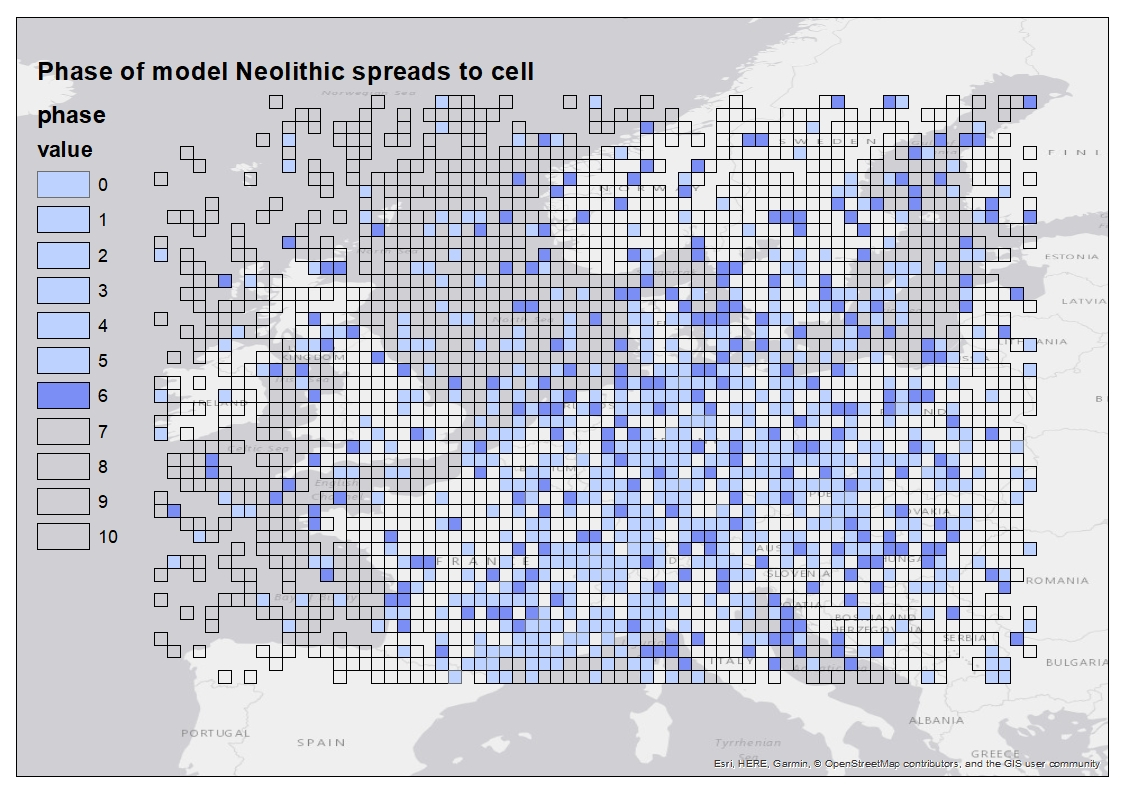
\includegraphics[width=0.8\textwidth]{figures/model-6}
	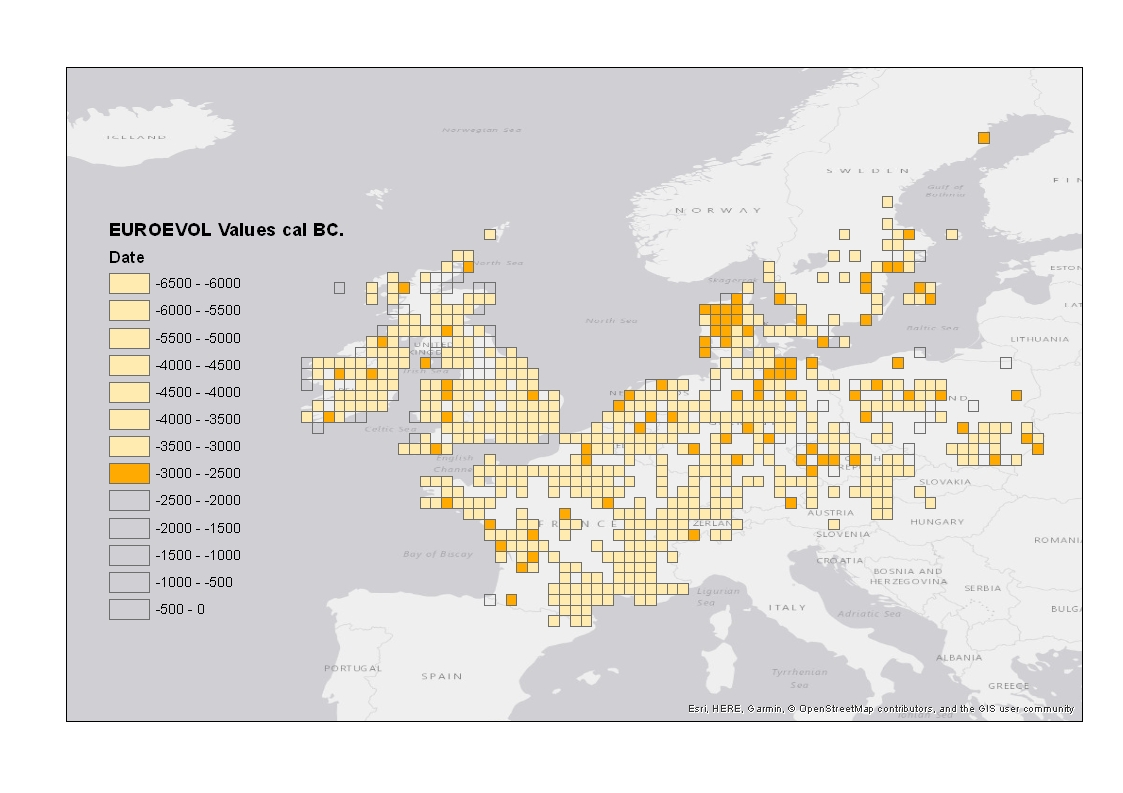
\includegraphics[width=0.8\textwidth]{figures/euroevol-6}
  \caption{Model state after phase six and corresponding EUROEVOL data}
  \label{fig:compare6}
\end{figure}

\begin{figure}
\centering
	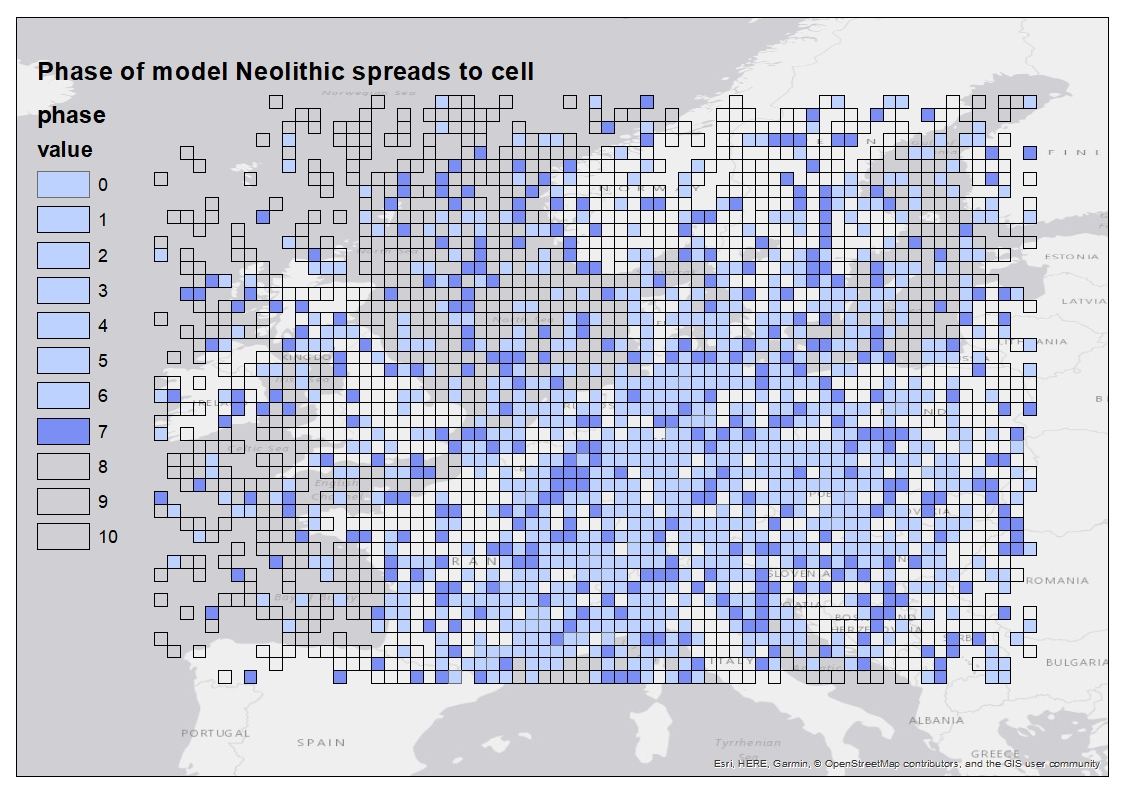
\includegraphics[width=0.8\textwidth]{figures/model-7}
	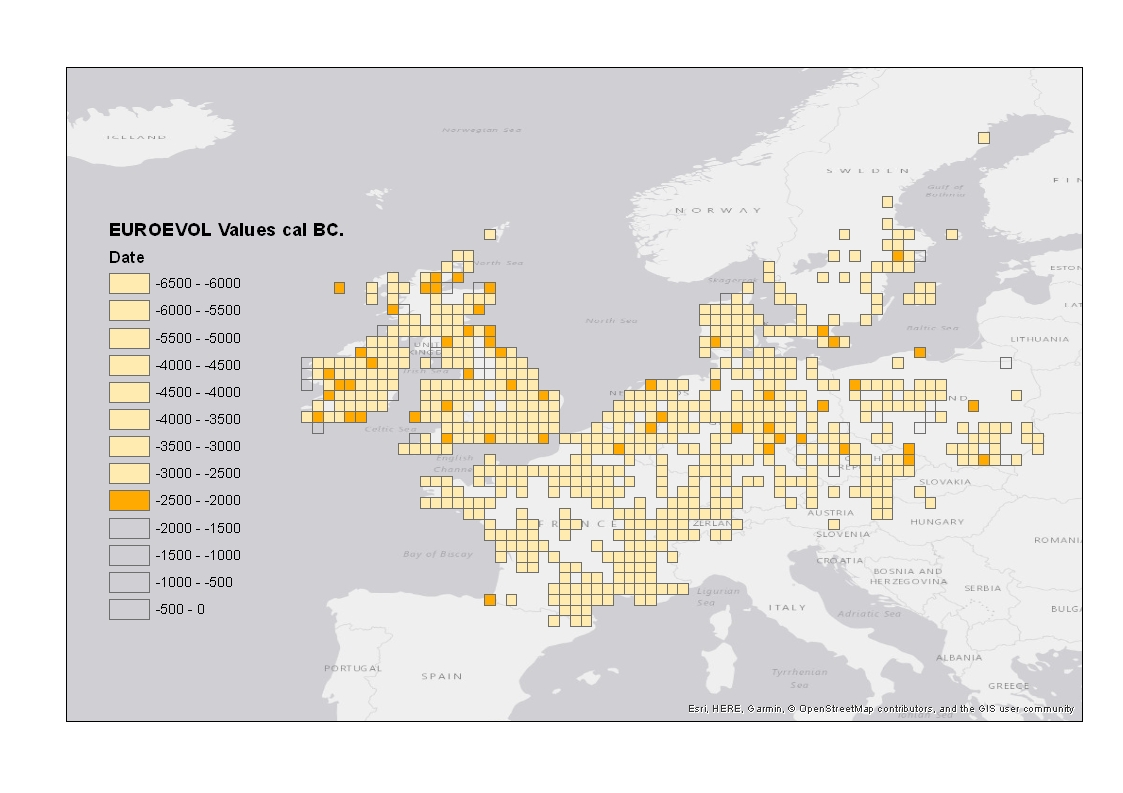
\includegraphics[width=0.8\textwidth]{figures/euroevol-7}
  \caption{Model state after phase seven and corresponding EUROEVOL data}
  \label{fig:compare7}
\end{figure}

The other category of conclusions that can be drawn from the model are inferences about the process that generated the data set, in this case the spread of the Neolithic. Clearly such a simplistic model is unlikely to provide any particularly ground breaking conclusions, but as a tool for EDA it can suggest further areas of interest. A particularly clear deviation between model and data set occurs for northern France and the British Isles, which have relatively well populated data sets. This deviation starts of in figure~\ref{fig:compare2}, gathers pace through figures~\ref{fig:compare3}, \ref{fig:compare4} and \ref{fig:compare5} and by figure~\ref{fig:compare6} there is a well established focus of Neolithic cells in the British Isles that is not matched in the model. This would suggest that another process is responsible for generating this part of the data set, a process that includes the long distances covered in figure~\ref{fig:compare2} to the north of Scotland and south-east of Ireland. Another difference is the spread up the west coast of France and along the north coast of France, through the low countries and across to Denmark. This spread appears to move much more rapidly, along the coast then the movement north and west in the model. This is perhaps a facet of the data and modelling process, or perhaps due to both the barrier and relatively rapid transport offered by the coast, or perhaps a combination of the both. 

\begin{figure}
\centering
	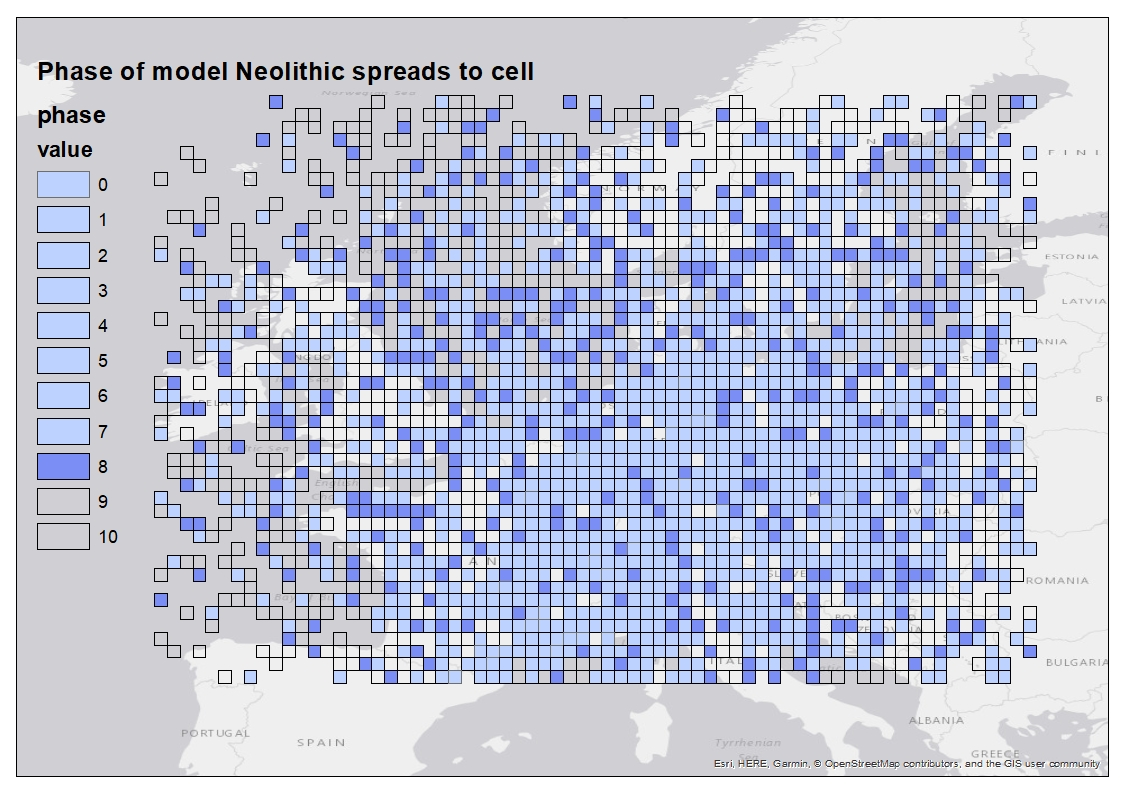
\includegraphics[width=0.8\textwidth]{figures/model-8}
	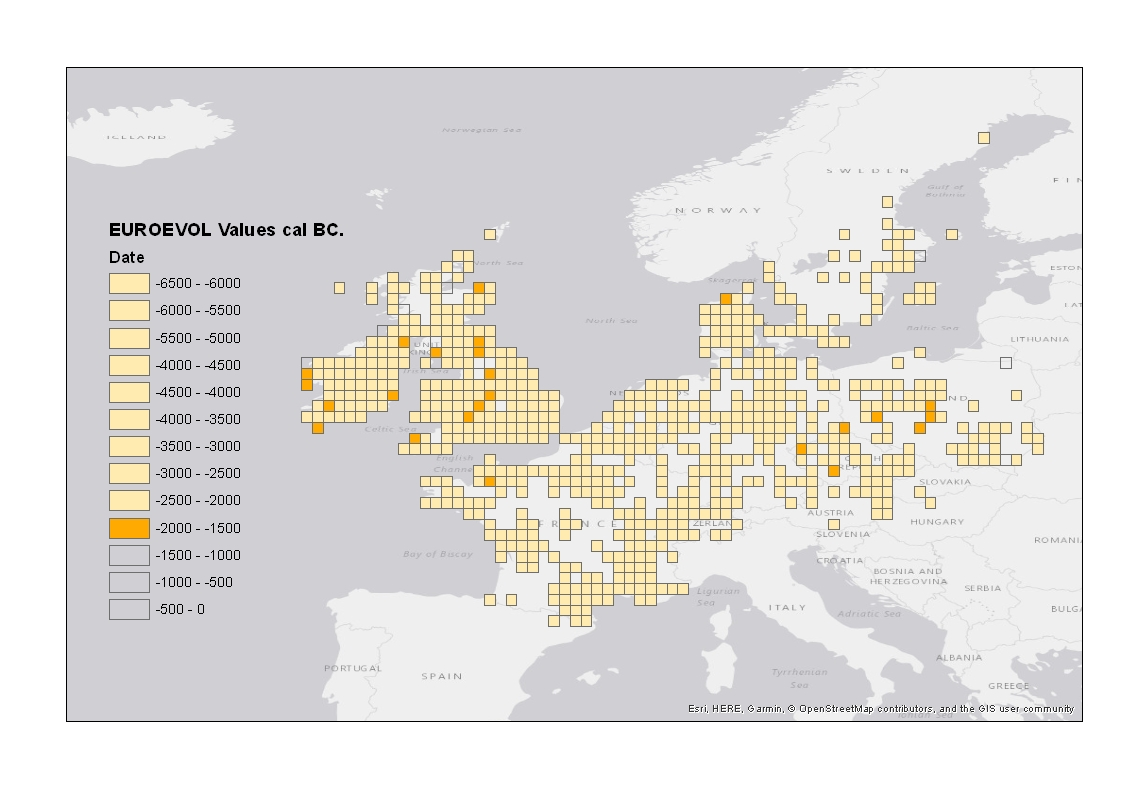
\includegraphics[width=0.8\textwidth]{figures/euroevol-8}
  \caption{Model state after phase eight and corresponding EUROEVOL data}
  \label{fig:compare8}
\end{figure}

\begin{figure}
\centering
	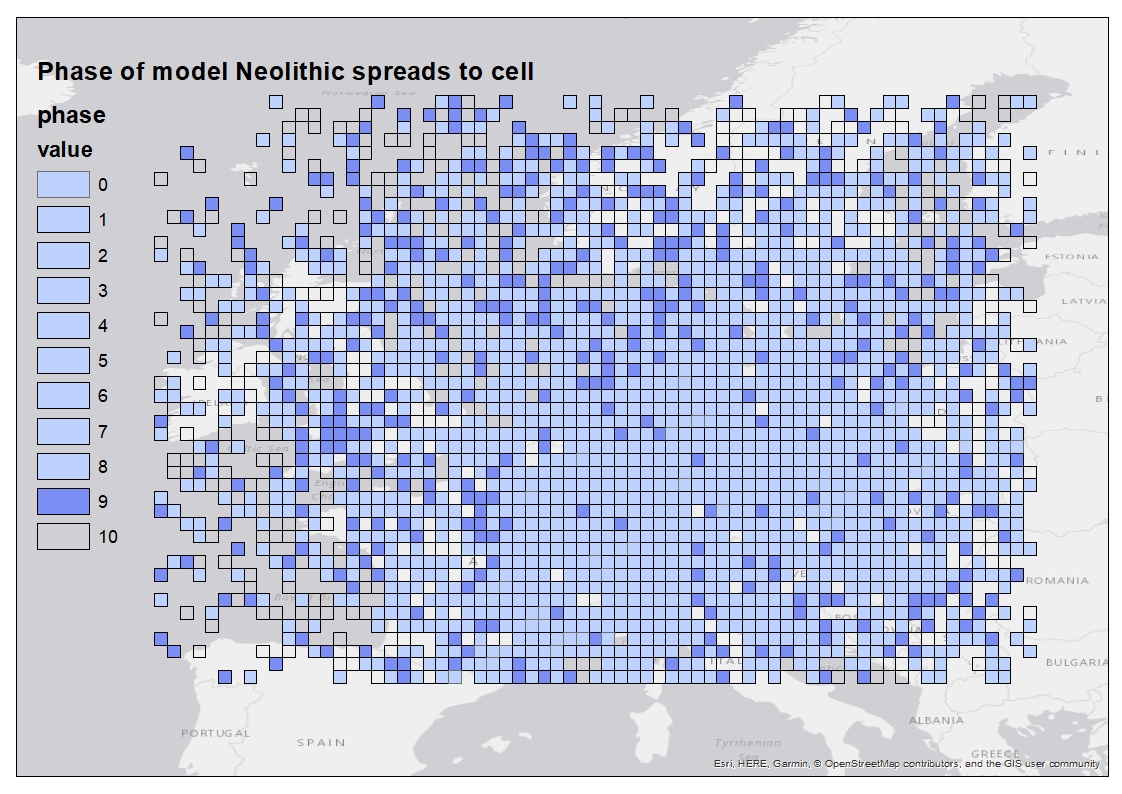
\includegraphics[width=0.8\textwidth]{figures/model-9}
	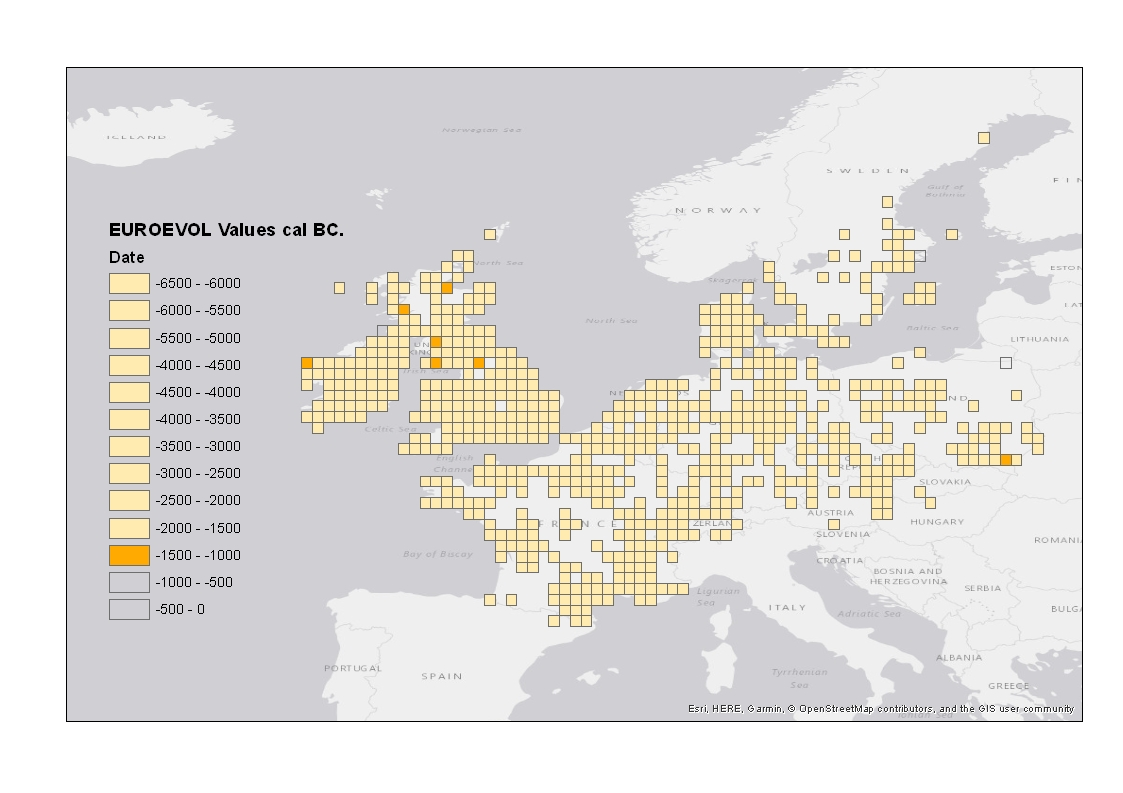
\includegraphics[width=0.8\textwidth]{figures/euroevol-9}
  \caption{Model state after phase nine and corresponding EUROEVOL data}
  \label{fig:compare9}
\end{figure}

This difference in France has been picked up by other studies, such as \citet{gkiasta2003neolithic} who put the difference down to different process, culture adoption by Mesolithic populations in the south and a spread of LBK cultures on the north \citep[60]{gkiasta2003neolithic}. The same study also notes and attempts to differentiate between the different processes that potentially make up the Neolithic transition. It is also noteworthy that \citet{gkiasta2003neolithic} appears to be based on a pre-cursor to the EUROEVOL dataset and that a cell based analysis, using earliest Neolithic dates per cell, has been undertaken. In this case it is used to create linear trend analysis \citep[54]{gkiasta2003neolithic}.

\begin{figure}
\centering
	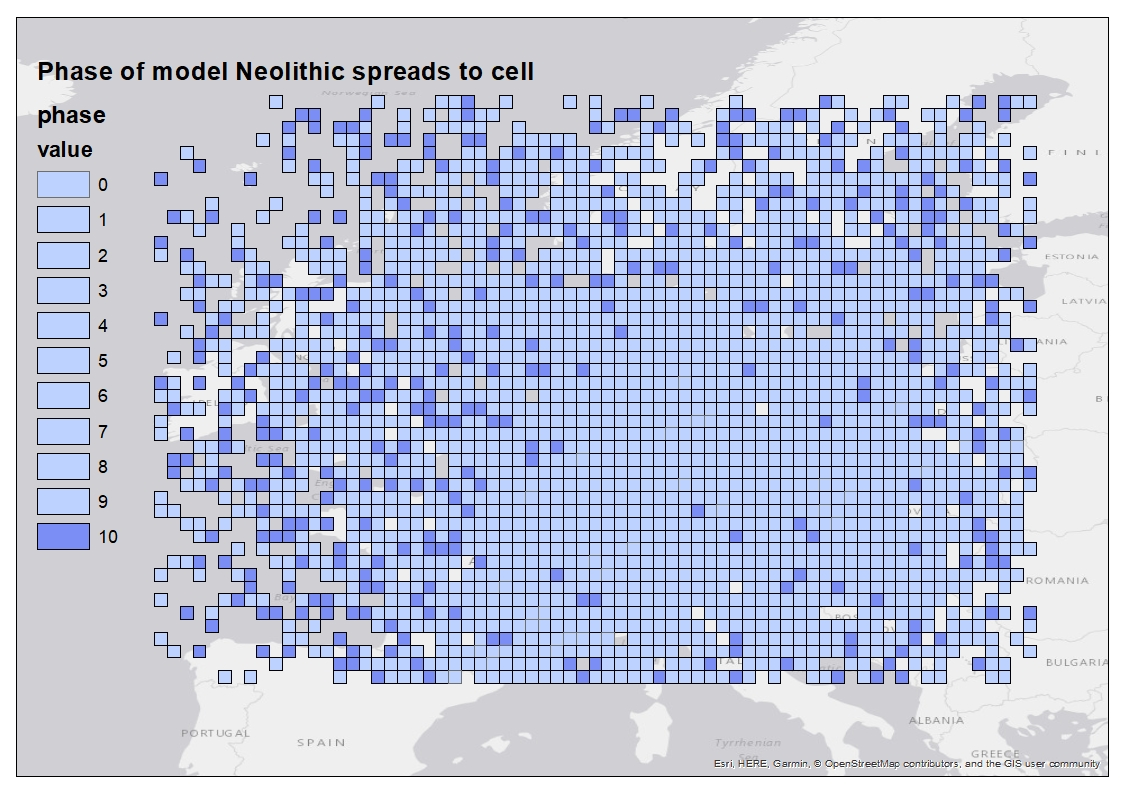
\includegraphics[width=0.8\textwidth]{figures/model-10}
	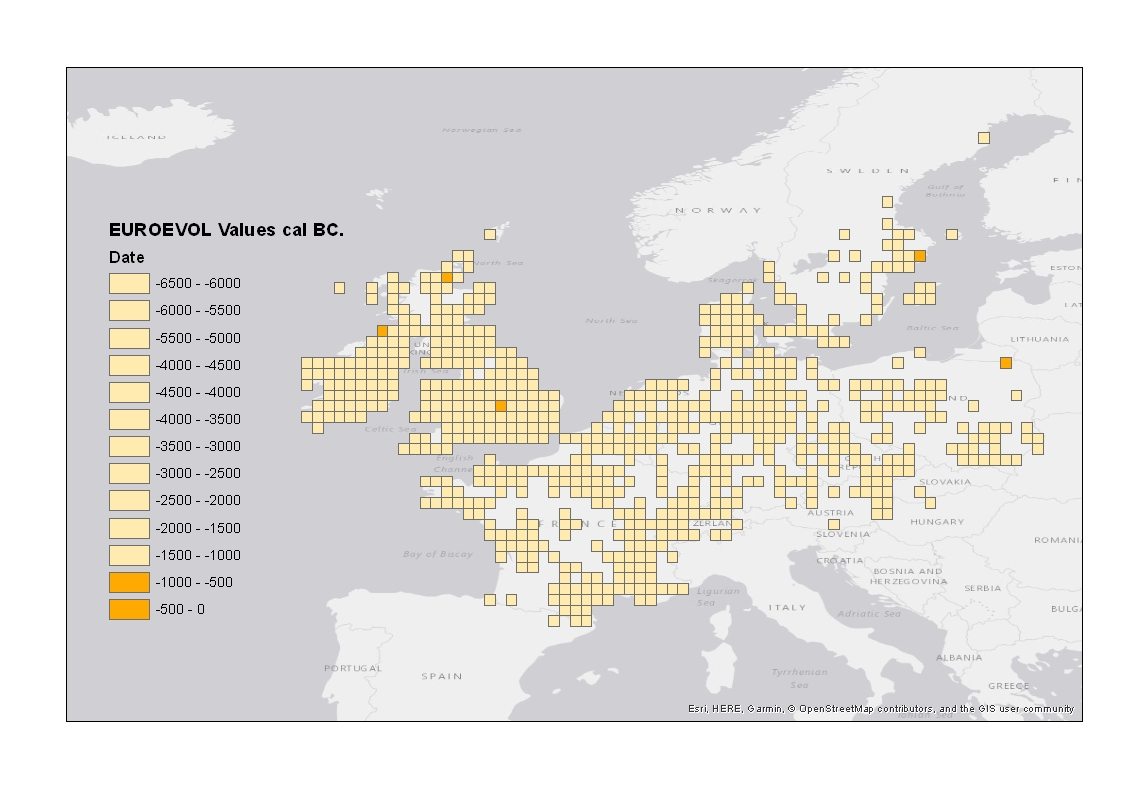
\includegraphics[width=0.8\textwidth]{figures/euroevol-10}
  \caption{Model state after phase ten and corresponding EUROEVOL data}
  \label{fig:compare10}
\end{figure}

\section{Conclusions}
This study has examined a large scale dataset, the EUROEVOL data set \citep{Manning:2016fk}, spread over a large spatial and temporal extent. So far the main use the data has been put to is determining population changes through Summed Probability Distribution techniques. These techniques were objectively reviewed, and found to be based on some unverified assumptions. Following this the particular application of these techniques to the EUROEVOL data was examined, a mathematical law was found to have been incorrectly treated as a claim to authority and the primary method of assessing the significance of the SPD approach was determined to be flawed. As part of this an assessment was made on the nature of the data and following that a brief review was made of the various different forms of analysis that archaeologists employ on pre-existing data sets.

The outcome of this review was to undertake a process of Exploratory Data Analysis on a simplified abstraction of the data set, using cells with the value of the earliest Neolithic date present in them, not the first time such an abstraction has been used. Unlike with previous work on this data set (see \citealp{gkiasta2003neolithic}) the distribution was not immediately assumed to be down to the original process of Neolithic transition, despite the clear patterns visible (e.g. in figure~\ref{fig:euroevol-detailed1}). The data set itself was put under the spotlight and found to contain omissions, including later values for the start of the Neolithic that one might expect. This was put down to the differential nature of archaeological investigation and highlights a facet of working with such large data sets. Had the cell size been larger, there would have been fewer erroneously late cells, but the resolution of the analysis would have been smaller and some of the more nuanced pattern of spread would have disappeared. Fundamentally this is a problem with such a fragmentary data set: how to deal with gaps in our knowledge? The approach above of simply taking the data at face value is clearly not always the most appropriate, an alternative approach would be to estimate values from some form of surrogate data. Such an approach is risky and would ideally be based around an interpretative process.

The next step in attempting to understand more about the creation of the dataset was to model it via a simulation. An analogy was drawn with epidemiology and cellular automata chosen as a modelling strategy based upon its relative success in that field. The process of modelling, in particular the types of transmission and the rates of transmission threw up interesting questions about the data set and the Neolithic transition, especially around the long distance `leapfrogging' required. This is likely due to both the fragmentary nature of the data set, but also reflects the potential for long distance travel (over land and across water). This is most obvious in the data set as sea travel, (e.g. figure~\ref{fig:compare2}) but there is clearly also the potential for travel by river. Finally the results of the model itself, when compared to the original data set show a reasonable comparison over large parts of the area covered by the data set, but clear divergence in other areas. These divergent areas would require a more nuanced, or even entirely separate model, suggesting clear regional differences, potentially due to differences in the process of Neolithic transition (but also potentially influenced by other, post-depositional processes). It is interesting to note that the biggest divergence is in the British Isles, the model assumes a continuous surface, which clearly the British Channel removes. It is not un-reasonable to conclude that this separation from the European mainland resulted in the Neolithic transition taking a different shape as it spread into Britain, with these differences at least in part down to the different nature of travel required.

This chapter has focused on the data, it has done so un-apologetically. As it is the data that is used to derive and make archaeological inferences, it is important we understand as much as possible about that data. In this case the data encompasses both spatial and temporal dimensions,  the true benefit of which can only be realised by combined spatio-temporal analysis. The SPD analysis was temporally focused, only treating the spatial component of the data as broad regions.
This is in contrast to the EDA and ensuing model, which considers the true nature of the data. While the use of a single value for the radiocarbon distribution is not ideal as it is only one potential value the date could take, it is a necessary simplification in order to perform analysis on such a large data set using relatively simple procedures. In many ways the complexity of the modern SPD approach creates an opacity around it, the complexity shrouds the fundamental issues with the data via statistical laws and significance tests. Results drawn from simpler, combined spatio-temporal methods, which are sympathetic to the data set are clearly more valuable.